w% !TeX root = ../main.tex

\chapter{HALF设备保护系统的设计}

\section{HALF预研工程}

合肥先进光源(Hefei Advanced Light Facility,HALF)是由国家同步辐射实验室提出的第四代基于衍射极限储存环(Diffraction Limited Storage Ring,DLSR)的同步辐射光源,HALF是一个位于中低能区,以真空紫外和软X射线为主的,具有高亮度、低发射度和唯一全辐射谱段空间相干性最先进的衍射极限光源。HALF将集成与相干性密切关联的系列先进测量技术,具有超快时间分辨、超高空间分辨和超高能量分辨的能力,为量子信息与量子材料、能源与环境、物质科学、生命科学等前沿研究领域提供强有力的研究平台。

HALF的设计定位世界领先,在技术上极具挑战,开展预研十分必要。目前国家同步辐射实验室在中国科学院和地方政府的共同支持下开展了HALF预研工程,预研工程将对加速器、光束线站的核心关键技术进行攻关及样机研制,为未来HALF的建设打好技术基础。HALF预研工程计划于2020年完成,目前最新设计的合肥先进光源的结构如图~\ref{fig:half-arch}所示,HALF由注入器、存储环和光束线站组成。

\begin{figure}[!htb]
	\centering
	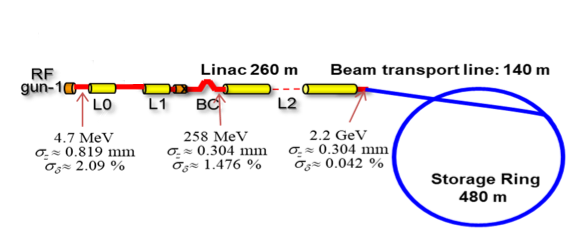
\includegraphics[width=0.9\textwidth]{half-arch.png}
	\caption{HALF总体结构图}
	\label{fig:half-arch}
\end{figure}

注入器由满能量直线加速器(Linac)和束流输运线(Beam transport line)组成,直线加速器用于产生电子,并将其加速至2.2GeV的能量,直线加速器有$L_{0}$到$L_{2}$三个加速段,各加速段的束流长度($\sigma_{z}$)和能散( $\sigma_{\delta}$)都标注在图~\ref{fig:half-arch}上。输运线负责将直线加速器的电子传输到存储环,沿储存环切线方向产生的同步辐射光通过光束线传输到实验站进行各种科学实验。

HALF存储环的光束发射度非常小,因此光束线可以将一定波长范围内的光束聚焦到其衍射极限,这种类型的存储环称为衍射极限存储环,HALF衍射极限存储环的最新设计参数如表~\ref{table:4.1}所示。

\begin{table}[!htb]
	\centering\small
	\caption{HALF储存环主要参数值}
	\label{table:4.1}
	  \begin{tabular}{ccc}
		  \toprule
		  参数        & 数值 & 单位\\
		  \midrule
		  能量  &  2.2  & GeV \\
		  周长  & 480  &  m \\
		  周期数  & 20 & - \\
		  自然发射度  & 85.1  &  pm $\cdot$ rad \\
		  工作点(H/V)  & 48.175/17.175  & - \\
		  自然色品  & -75, -79  &  - \\
		  动量紧缩因子   & $6.3\times 10^{-5}$  &  - \\
		  阻尼分配数(H/V/L)  &  1.475/1.0/1.525  & -  \\
		  自然阻尼时间(H/V/L)  & 22/32.4/21.2  & ms \\
		  电子单圈弯铁辐射能量损失 & 217.5  &  keV \\
		  自然能散  & $0.66\times 10^{-3}$   & - \\
		  直线节数目  & 40个(20个长直线节+20个中直线节)& - \\
		  长直线节长度  & 5.5& m \\
		  长直线节中点处的$\beta_{x}$/$\beta_{y}$/色散函数 & 5.445/2.533/0.0 & m \\
		  中直线节长度  & 2.2 & m \\
		  中直线节中点处的$\beta_{x}$/$\beta_{y}$/色散函数  & 2.842/1.954/0.028 & m \\
		  \bottomrule
	  \end{tabular}
\end{table}

\section{加速器中的设备保护系统}

\subsection{设备保护系统任务}
设备保护系统(Equipment Protection System,EPS)是加速器控制系统的重要组成部分,负责保护加速器的设备安全。EPS在加速器各分总体、系统间建立联锁保护逻辑,当设备出现故障时,EPS能够快速地对加速器重要设备实施保护,并向中央控制系统报告设备故障信息,对故障数据进行存档和分析。根据被控对象的不同,EPS可分为慢联锁保护系统(Slow Protection System,SPS)和快联锁保护系统(Fast Protection System,FPS)。从系统响应时间的角度来看,SPS的响应时间在10ms量级,而FPS的响应时间要求在10$\mu$s量级。SPS和FPS的具体保护场合如下:

\begin{enumerate}
  \item SPS监测的设备状态信号主要是真空度、温度、冷却水流量等与设备运行安全相关的信号,经过SPS联锁逻辑判断后,迅速实施相应的设备保护措施。

  \item FPS的保护场合是在加速器运行过程中,如果发生了束流偏离轨道达到一定阈值或者某些设备出现故障,导致电子束流可能会损毁机器,此时必须采取保护措施及时切断束流。
\end{enumerate}

一般来说,SPS和FPS是相对独立的两个系统,分别采用相互独立的通信网络和硬件设备,本章主要描述响应时间在10ms量级的设备慢联锁保护系统相关设计。

\subsection{国外加速器EPS调研}
本节对国外加速器装置的EPS进行了调研,国际上的加速器装置习惯将设备保护系统称为机器保护系统(Machine Protection System,MPS),主要关注EPS的系统结构和硬件组成。

\subsubsection{LCLS的机器联锁保护系统}

直线加速器相干光源(Linac Coherent Light Source,LCLS)是世界上第一个发射硬X射线的自由电子激光装置,长130米,位于美国斯坦福直线加速器中心。LCLS机器保护系统的任务是避免波荡器等重要设备受到束流照射而损坏,要求MPS在一个束流脉冲周期8.33ms内切断束流。MPS监测的信号包括束流损失信号、束流位置信号、束流强度和光束线插入件状态。

\begin{figure}[!htb]
	\centering
	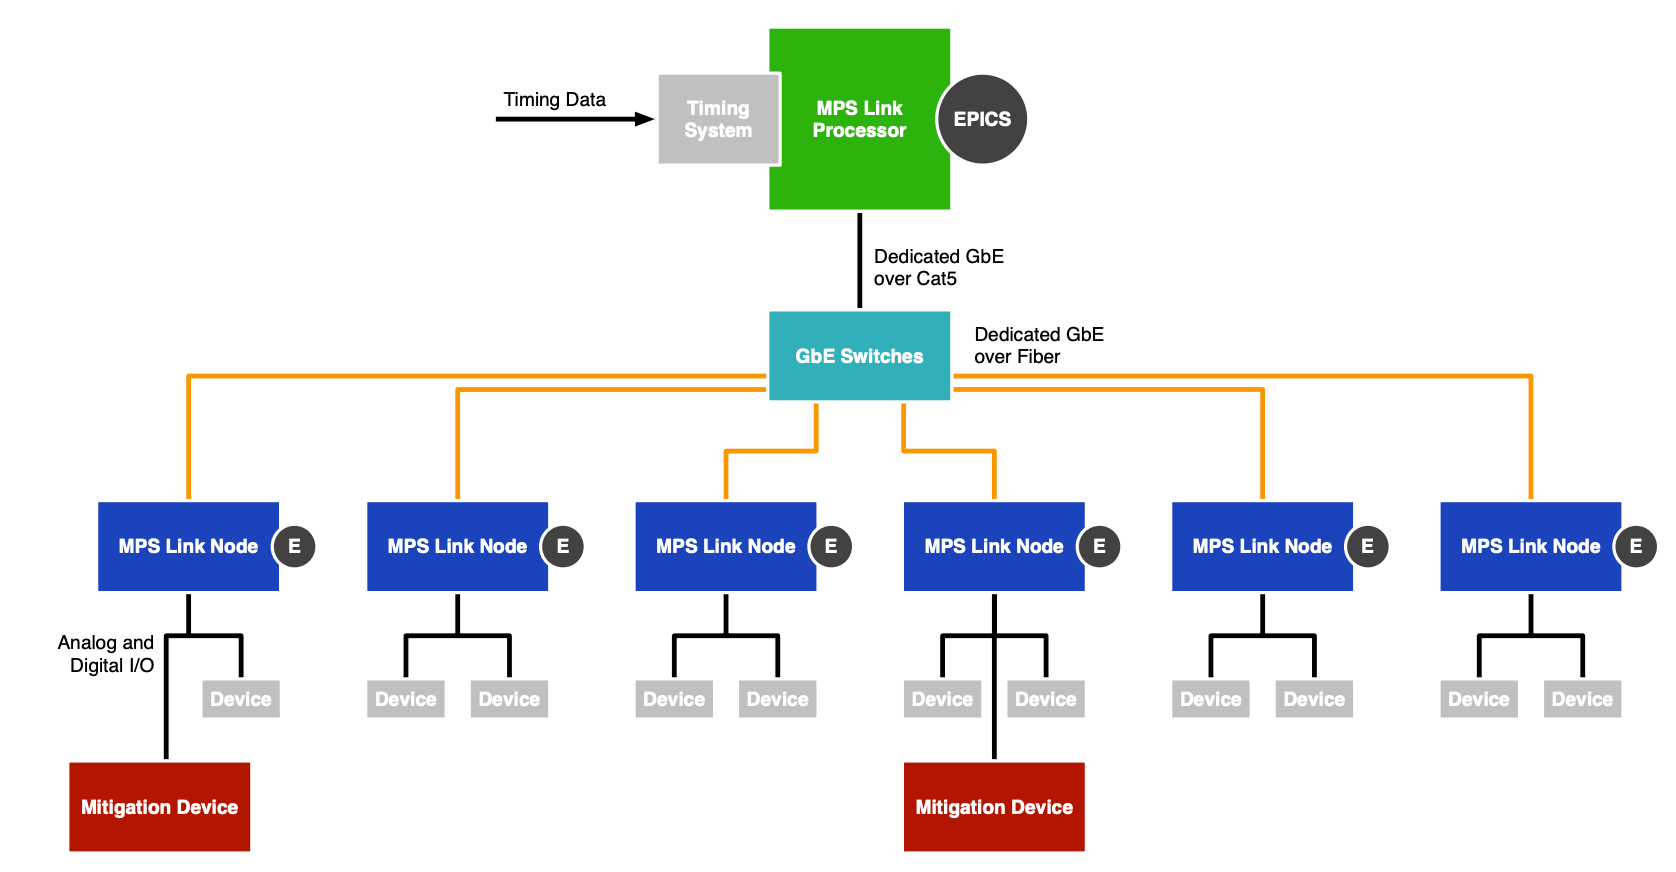
\includegraphics[width=\textwidth]{lcls-eps-arch.png}
	\caption{LCLS机器保护系统结构图}
	\label{fig:lcls-eps-arch}
\end{figure}

LCLS MPS的系统架构如图~\ref{fig:lcls-eps-arch}所示,MPS由32个连接节点(Link Node)和一个中央处理器(Link Processor)组成,节点采用千兆光纤以太网通过核心交换机与中央处理器连接成星型拓扑结构,通信协议是LCLS自主设计的实时协议。连接节点分布于从激光注入器到X射线实验线站的整个装置,负责接收束流故障信号,中央处理器按照联锁保护逻辑处理来自节点的束流故障信号,通过相应的设备(Mitigation device)切断束流。中央处理器和连接节点同时接入到EPICS控制网络,用于中控系统监控MPS状态。

MPS连接节点基于型号为Xilinx Vertex4的FPGA芯片实现,每个连接节点可支持多达96路数字输入,8路固态继电器输出,4路TTL兼容逻辑电平触发输入和4路触发输出,同时配备了单独的串口与EPICS IOC通信。

\subsubsection{RAON的机器联锁保护系统}

Rare isotope Accelerator complex for ON-line experiment(RAON)是一台正在建设中的重离子加速器,为在线同位素分离实验和飞行时间型碎片分离实验提供平台。RAON由韩国基础科学研究所(IBS)负责,CERN,Fermilab,TRIUMF等实验室也共同参与到RAON项目建设中。

\begin{figure}[!htb]
	\centering
	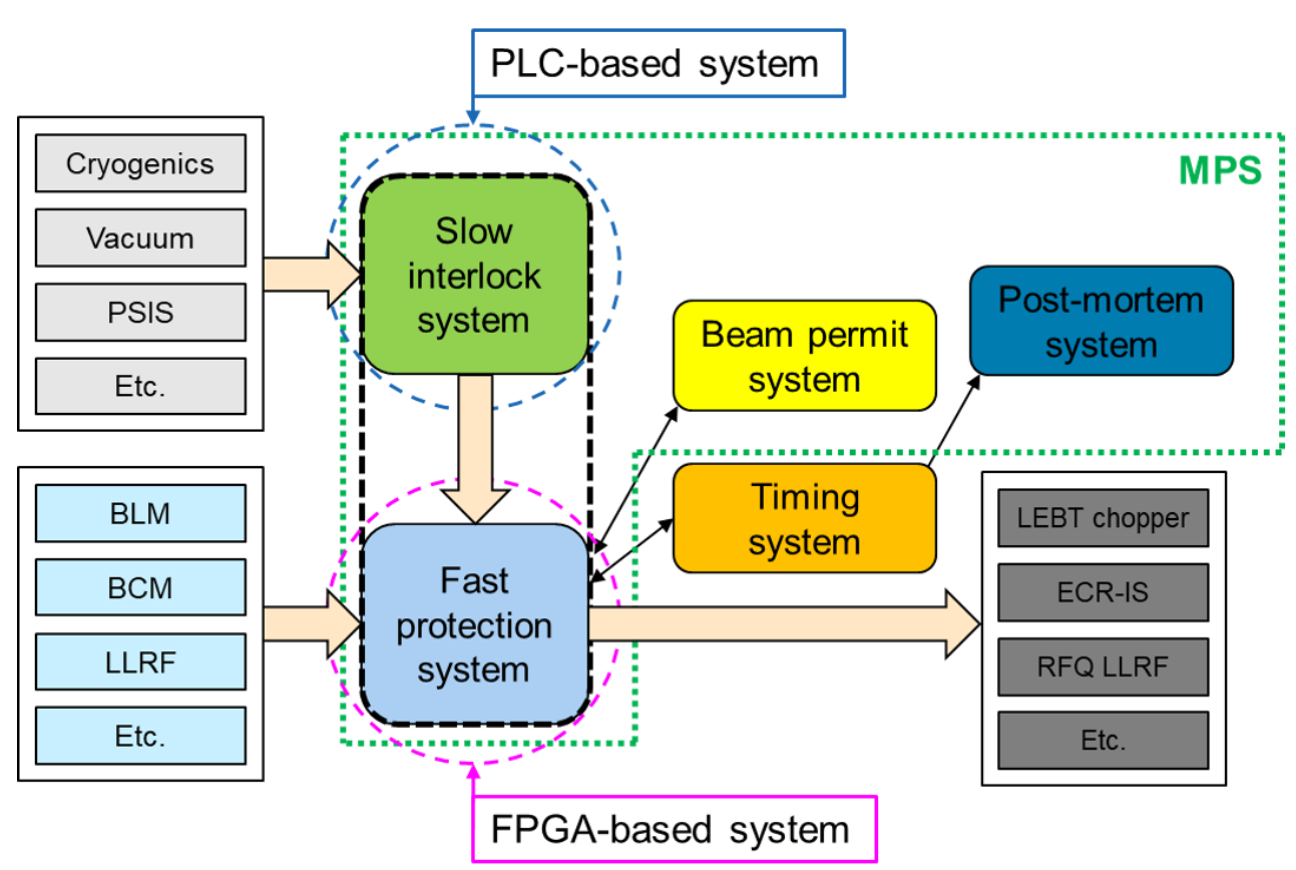
\includegraphics[width=\textwidth]{RAON-eps-arch.png}
	\caption{RAON机器保护系统结构图}
	\label{fig:RAON-eps-arch}
\end{figure}

RAON的MPS结构如图~\ref{fig:RAON-eps-arch}所示,由Slow Interlock System(SIS)、Fast Protection System(FPS)、Beam Permit System(BPS)和Post-mortem System(PMS)组成,各系统具体设计如下:

\begin{enumerate}
  \item SIS基于PLC实现,监测低温,真空等系统中的设备信号,一旦设备出现故障,SIS要在几十ms内通过FPS实施切断束流的设备保护措施。

  \item FPS各节点基于FPGA实现,FPS节点监测的信号来自束流丢失监测器(BLM)、束流流强监控器(BCM)、低电平(LLRF)系统设备等,FPS需要在几十$\mu$s,通过禁止高频功率输出等措施切断束流。

  \item BPS负责根据加速器不同的运行模式来切换MPS运行状态。

  \item PMS是用来对设备故障信号进行存档和分析的系统。

\end{enumerate}

\subsection{设备保护系统的结构}

EPS分布于整个加速器装置,在结构上有分布式处理和和集中式控制的特点,具体来说:

\begin{enumerate}
  \item 分布式处理:EPS在前端层是完全分布式的。加速器各系统设备状态都有专门的EPS控制器负责监测,一旦监测到设备出现故障后,要迅速将故障信息传输至主控制器进行联锁保护。
  \item 集中式控制:从控制角度上说,EPS是集中式的。主控制器协调整个EPS的运行,处理各种级别的联锁保护,同时负责将EPS收集到的设备故障信息上报到中央控制系统。
\end{enumerate}

\section{HALF设备保护系统设计}

作为HALF控制系统的重要组成部分,EPS的任务是在HALF不同的运行模式下保证机器设备的安全。HALF EPS在HALF各分总体、系统间建立联锁保护逻辑,监测的设备状态主要包括真空度、温度、冷却水流量等,在经过系统联锁逻辑判断后,给出禁止电子枪触发、禁止RF功率输出允许、禁止注入与引出等联锁保护信号。HALF EPS遍布整个装置,联锁输入信号分布广泛,数量众多,包括各设备状态信号和来自其他系统的联锁信号,具体如下:

(1)真空泄漏信号;

(2)真空阀门状态信号;

(3)储存环真空室温度信号;

(4)磁铁以及磁铁电源状态信号;

(5)冷却水温度和流量信号;

(6)微波设备状态信号;

(7)速调管反射功率信号;

(8)束流测量系统联锁信号;

(8)来自人身安全系统的联锁信号;

(9)屏蔽间门状态信号;

(9)来自光束线站的联锁信号;

(10)消防信号和中控急停信号。

EPS通过给出某些设备的禁止运行信号从而达到保护重要设备的目的,保护措施具体如下:

(1)禁止电子枪触发;

(2)禁止固态放大器触发;

(3)禁止调制器触发;

(3)禁止高频功率输出;

(3)禁止储存环注入。

根据HALF的体系架构,我们可将HALF EPS由上至下分为总体级联锁、分总体级联锁、系统级联锁三个联锁层次,其中,下层系统为上层联锁提供信号,并接收来自上层的联锁保护命令。三个层次的联锁功能具体如下:

\begin{enumerate}
  \item 总体级联锁:根据HALF的不同运行模式切换EPS的运行模式;处理HALF各分总体之间的联锁关系,以及接收来自人身安全系统等外部系统的联锁信号,确保整个HALF的运行安全。

  \item 分总体级联锁:负责分总体内各个系统之间设备的联锁保护,保证分总体的安全运行,同时向总体级联锁提供联锁输入信号。

  \item 系统级联锁:负责各系统内部设备的联锁保护,保证分系统运行正常,并向分总体级联锁系统报告设备故障信息和联锁保护信息。

\end{enumerate}

\subsection{HALF EPS运行模式}

运行管理系统负责对HALF的运行状态进行管理,EPS需要接受来自运行管理系统的命令,切换自身的运行模式以匹配不同的HALF运行状态。HALF EPS设计了5个运行模式,分别如下:

\begin{enumerate}
  \item 停机模式:此模式下HALF处于停机状态,EPS需要确保所有真空阀门和光束线前端区的光闸均处于关闭状态,并停止除束测系统以外所有系统设备的定时触发信号。

  \item RF老练模式:HALF处于RF老练模式下时,EPS需要开启对微波设备的联锁保护状态。

  \item 注入器调试模式:此模式下仅进行注入器分总体的束流调试,注入器EPS正常开启,旁路掉储存环EPS、光束线EPS的联锁输入信号。

  \item 储存环调试模式:此模式下进行注入器和储存环的束流调试,注入器EPS和储存环EPS正常开启,旁路掉光束线EPS联锁输入信号。

  \item 运行模式:HALF处于正常的运行状态,此时EPS开启全部联锁保护功能。

\end{enumerate}


\subsection{HALF EPS总体结构}

\begin{figure}[!htb]
	\centering
	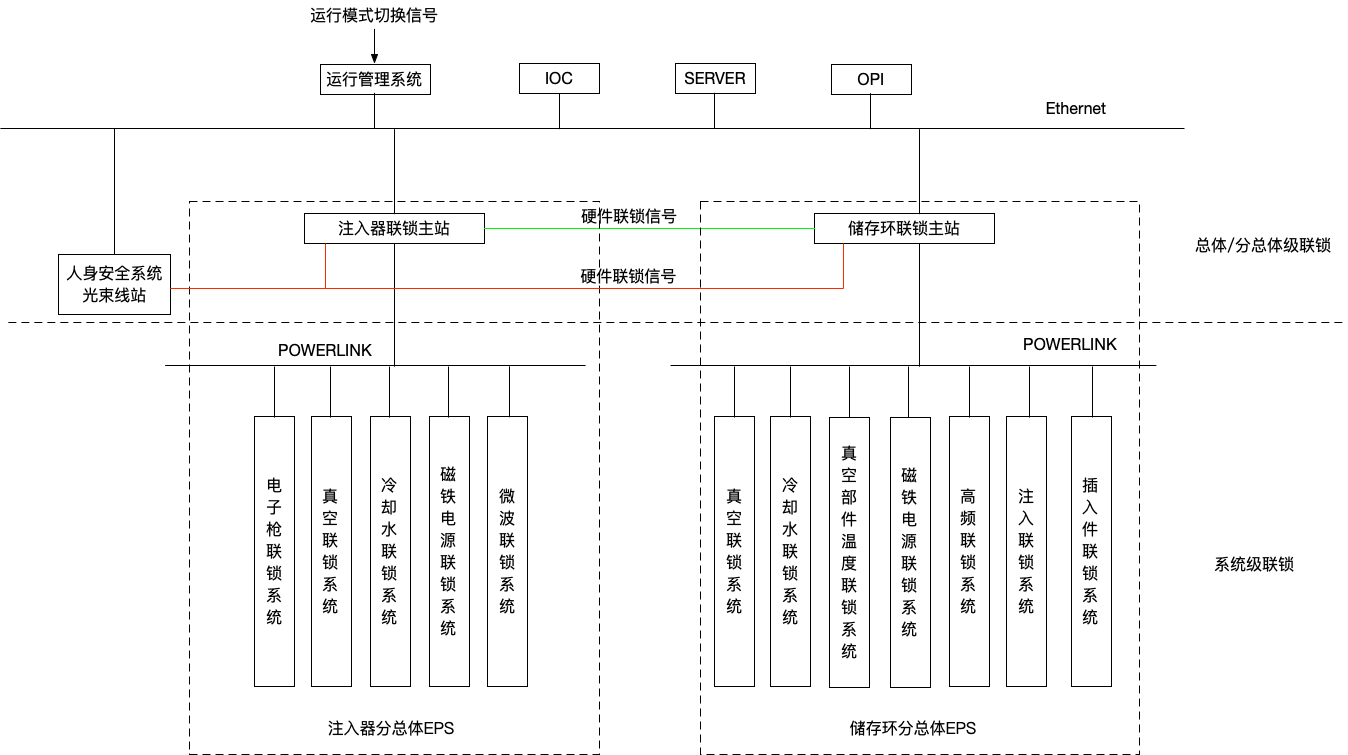
\includegraphics[width=\textwidth]{halfeps-arch.png}
	\caption{HALF EPS总体结构图}
	\label{fig:halfeps-arch}
\end{figure}

根据HALF的体系架构和EPS的联锁等级,我们设计了如图~\ref{fig:halfeps-arch}所示的HALF EPS总体结构,其结构可以概括如下:

\begin{enumerate}
  \item HALF EPS可以分成注入器分总体EPS和储存环分总体EPS两部分,分总体EPS由各子系统EPS组成,负责本分总体范围内的设备安全。其中注入器分总体EPS包括了电子枪EPS、真空EPS、磁铁以及磁铁电源EPS、微波EPS、冷却水EPS和触发控制系统,储存环分总体EPS包括了真空单元EPS、注入EPS、磁铁以及磁铁电源EPS、高频EPS、插入件EPS、冷却水EPS、光束线前端EPS。

  \item 各分总体EPS由一个主控制器和多个从控制器组成,其中主控制器负责处理本分总体内各个系统之间的联锁逻辑,从站作为分总体内各系统EPS控制器,负责收集并处理系统内的设备联锁故障信号,同时将从站监测的故障信号上传至主站,供主站进行分总体或者总体级的联锁处理。

  \item 两个分总体EPS的主站控制器通过快速光纤或硬件信号连接,处理分总体之间的总体级联锁保护关系。

  \item 来自人身安全系统等外部系统的联锁信号采用硬件信号的形式接入分总体EPS主站控制器,通过相应的分总体EPS实施保护。

  \item 来自运行管理系统的控制命令采用硬件信号的形式接入EPS,根据不同的HALF运行状态,EPS将切换不同的联锁模式。

  \item EPS通过千兆以太网接入HALF控制系统,将设备故障信息和联锁保护信息通过IOC上传至HALF中控系统,同时接受来自中控系统的控制命令。
\end{enumerate}

\subsection{HALF EPS实现方案}

根据HALF EPS的联锁保护需求和总体结构,我们可以采用POWERLINK作为分总体EPS的通信网络,Zynq控制器作为EPS的前端控制器。根据第三章对基于POWERLINK的分布式I/O系统的性能测试结果,千兆POWERLINK网络可以提供小于1ms的联锁保护,完全满足EPS小于10ms的联锁保护响应时间需求;Zynq控制器的信号处理时间为5$\mu$s,也为快联锁保护系统提供了可行性方案。和基于PLC的硬件联锁系统相比,采用POWERLINK实时以太网和Zynq控制器的EPS可以提高系统的实时性和信号处理的速度,同时避免了硬件联锁系统布线复杂的问题。具体实现方案如下:

如图所示,各分总体EPS基于独立的POWERLINK网络设计,主站控制器和从站控制器均采用Zynq控制器,从站控制器负责收集本系统内的设备状态信号,通过POWERLINK传输至主站控制器,经过主站控制器内预设的联锁逻辑处理之后,再通过POWERLINK网络传输至相应的本分总体从站输出保护动作,或者通过快速光纤传输至其他分总体EPS实施保护动作。

从站方案设计:
从站控制器作为分总体内部的系统控制器,保护任务如下:

(1)负责系统内设备的联锁保护,系统内与联锁相关的设备信号直接接入从站控制器,经过从站内的控制逻辑处理单元处理后,直接通过相应设备或系统输出保护动作。

(2)接收通过POWERLINK网络接收来自主站保护命令,从而实施保护。

主站方案设计:
分总体EPS主站需要协调整个EPS的运行,接收并处理的联锁信号较多,具体如下:

(1)处理来自各POWERLINK从站的分总体内部设备联锁信号,通过分总体内相应从站输出保护动作,或者通过硬件联锁信号传输至其他分总体EPS实施保护动作;

(2)接收来自其他分总体EPS的硬件联锁信,通过本分总体内相应从站实施保护动作号;
  		
(3)接收来自人身安全系统等外部系统的硬件联锁信号,通过分总体内相应从站实施保护动作;

(4)接收来自运行管理系统的硬件控制信号,切换EPS运行模式;

(5)通过千兆以太网与IOC通信,将设备故障信息和联锁保护信息通过IOC上传至HALF中控系统,同时接受来自中控系统的控制命令。

下面分别对HALF注入器、储存环、光束线三个分总体EPS的设计进行阐述。

\section{注入器EPS设计}

HALF注入器的输出能量为2.2Gev,为满能量注入器。注入器包括直线加速器和输运线,其中直线加速器的长度为260米,输运线长度为140米。注入器分总体由电子枪系统、真空系统、微波系统、磁铁电源系统、冷却水系统、束流测量系统等组成,注入器的主要设备有电子枪、预聚束器和聚束器、加速管、聚焦磁铁组、束测设备、固态放大器、速调管、调制器。电子枪负责产生并加速电子束流,次谐波聚束器、聚束器的作用是将电子枪产生的空间分布均匀的电子束流进行聚集,并加速至接近光速。HALF注入器有三个加速段,每个加速段里有若干加速管,加速管负责加速电子束流至2.2Gev满能量。微波系统设备包括速调管、调制器、波导管等设备,速调管输出的微波功率经波导和耦合器分出部分功率馈入聚束器,速调管输出的剩余微波功率经波导功分器再馈入加速管。聚焦四级磁铁产生聚焦磁场用来聚束,聚焦四级磁铁组分布在电子枪出口和加速管末段。真空系统和冷却水系统分布于整个注入器,负责监控各设备真空度和冷却水温度流量的变化。

注入器的输运线由若干冲击磁铁、切割磁铁、二极磁铁、四极磁铁、校正磁铁组成,负责将直线加速器产生的束流传输到储存环注入点。

注入器EPS的任务是当注入器分总体内部设备出现故障或者接收到来自分总体外部的联锁故障信号时,在注入器分总体范围内,通过相应的系统实施设备保护措施。注入器EPS的功能可以总结如图~\ref{fig:linac-eps-arch}所示,

 \begin{figure}[!htb]
	\centering
	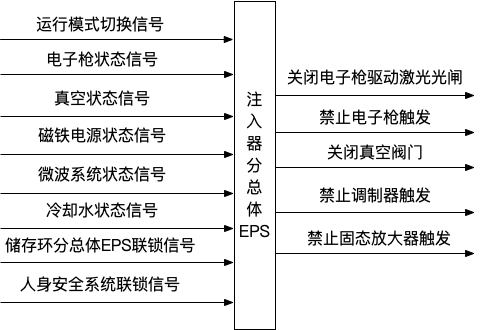
\includegraphics[width=0.8\textwidth]{linac-eps-arch.png}
	\caption{注入器EPS联锁保护功能图}
	\label{fig:linac-eps-arch}
\end{figure}

注入器EPS的输入联锁信号较多,包括来自注入器分总体本身的联锁信号,如微波设备状态信号等;其他分总体的联锁信号,如储存环分总体联锁信号;来自外部系统的联锁信号,如人身安全系统。对于不同的联锁信号,注入器EPS需要提供系统级、分总体级和总体级的联锁保护措施,注入器EPS的保护对象可以分为以下两类:
\begin{enumerate}
  \item 重要设备保护:当设备真空状态、冷却水温度与流量、速调管反射功率、外部联锁信号等出现故障时,注入器EPS通过禁止同步触发信号、关闭电子枪高压、关闭真空阀门等方式,保护电子枪、微波系统设备、储存环真空部件等重要设备。
  \item 人身安全保护:在隧道门禁、辐射剂量等信号指示注入器区域未满足人身安全要求情况下,注入器EPS通过禁止电子枪等各设备的同步触发信号,切断束流,防止现场工作人员遭受辐射伤害。
\end{enumerate}

注入器EPS由分总体下各系统EPS组成,每个系统EPS至少由一个Zynq控制器负责,各系统EPS配合工作,共同完成注入器EPS的联锁保护任务。各系统EPS控制器除了负责本系统内系统级的联锁保护,同时还需要将系统内的设备故障信号上传至POWERLINK主站,经过联锁逻辑处理后,禁止相应设备的同步触发信号来实施分总体级的联锁保护。注入器EPS各等级联锁保护的实现方式具体如下:
\begin{enumerate}
  \item 各系统EPS控制器负责收集本系统内部设备状态信号,经过控制器内置的联锁保护逻辑处理后,直接实施保护动作,这种属于系统级别的保护。
  \item POWERLINK主站根据注入器分总体内的设备故障信号,经过主站控制器的联锁保护逻辑处理后,通过切断定时触发器的同步触发信号来实施保护动作,这种属于分总体级别的保护。
  \item POWERLINK主站接收来自其他分总体或者外部系统的联锁故障信号,经过主站控制器的联锁保护逻辑处理后,通过切断定时触发器的同步触发信号来实施保护动作,这种属于总体级别的保护。
\end{enumerate}

对于一些重要的设备,EPS还会提供冗余保护措施。当重要设备发生故障时,EPS会直接执行快速的设备保护措施,同时会切断相应设备的同步触发信号,这两种联锁保护方式相互之间保持独立性,冗余安全性好。例如,当微波设备出现故障时,注入器EPS会采取禁止调制器功率输出和切断调制器定时触发信号的双重保护措施。

下面将分别阐述注入器各系统EPS的功能和设计。

\subsection{电子枪EPS}

电子枪EPS对于电子枪故障信号,采用关闭电子枪高压、关闭电子枪灯丝电源的方式来使电子枪停止出束;对于来自其他系统或分总体的设备故障信号,电子枪EPS采取禁止电子枪同步触发信号的方式来切断束流,以防止相应设备被电子束流打坏。电子枪EPS的联锁输入信号包括系统级联锁信号、分总体级和总体级联锁信号,具体的联锁保护功能总结如下:

\begin{figure}[!htb]
	\centering
	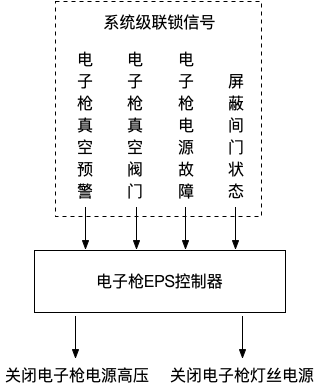
\includegraphics[width=0.45\textwidth]{e-gun-eps-system.png}
	\caption{电子枪EPS系统级联锁保护功能功能图}
	\label{fig:e-gun-eps-system}
\end{figure}

\begin{enumerate}
  \item 图~\ref{fig:e-gun-eps-system}所示的电子枪EPS系统级联锁保护功能,系统级联锁信号包括电子枪附近的真空阀门状态信号、电子枪真空度信号和屏蔽间门状态信号,联锁信号直接连接到电子枪EPS控制器进行处理。当真空阀门处于关闭状态时,或电子枪出现真空故障时,或屏蔽间门处于打开状态时,电子枪EPS控制器会直接采取关闭电子枪高压和电子枪电源的保护措施。

   \begin{figure}[!htb]
	\centering
	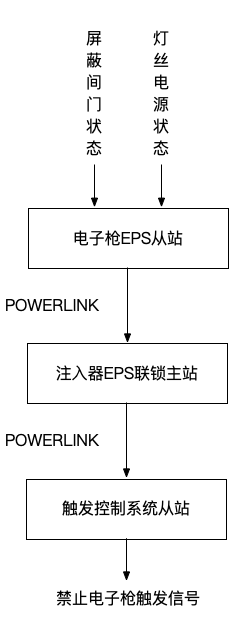
\includegraphics[width=0.7\textwidth]{e-gun-eps-global.png}
	\caption{电子枪EPS分总体级和总体级联锁保护功能图}
	\label{fig:e-gun-eps-global}
\end{figure}
 
  \item 图~\ref{fig:e-gun-eps-global}所示的电子枪EPS分总体级和总体级联锁保护功能,分总体级的联锁信号包括电子枪分总体内各设备的真空度信号、冷却水流量信号、屏蔽间门状态信号等,总体级的联锁信号包括来自储存环、光束线站分总体以及人身安全系统等外部系统的联锁信号。这些联锁信号经过主站的联锁逻辑处理后,通过电子枪EPS切断电子枪同步触发信号的方式来实施保护。

\end{enumerate}

\subsection{真空EPS}
注入器真空系统由若干台真空计和真空阀组成,真空计负责监测电子枪区、次谐波聚束器区、加速管区、波导管区、速调管区的真空度,真空阀门分别位于电子枪出口处和最后一个加速管出口处。真空EPS的联锁输入信号包括系统级联锁信号、分总体级联锁信号,具体的联锁保护功能总结如下:

\begin{figure}[!htb]
	\centering
	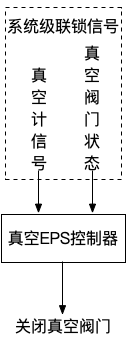
\includegraphics[width=0.15\textwidth]{linac-vacuum-eps-system.png}
	\caption{真空EPS系统级联锁保护功能图}
	\label{fig:linac-vacuum-eps-system}
\end{figure}

\begin{enumerate}
  \item 图~\ref{fig:linac-vacuum-eps-system}所示的真空EPS系统级联锁保护功能,系统级联锁输入信号包括真空计信号与真空阀门状态信号,系统级联锁信号直接连接到真空控制器中,真空控制器根据联锁故障信号判断设备的真空状态,做出关闭相应真空阀门的动作。

\begin{figure}[!htb]
	\centering
	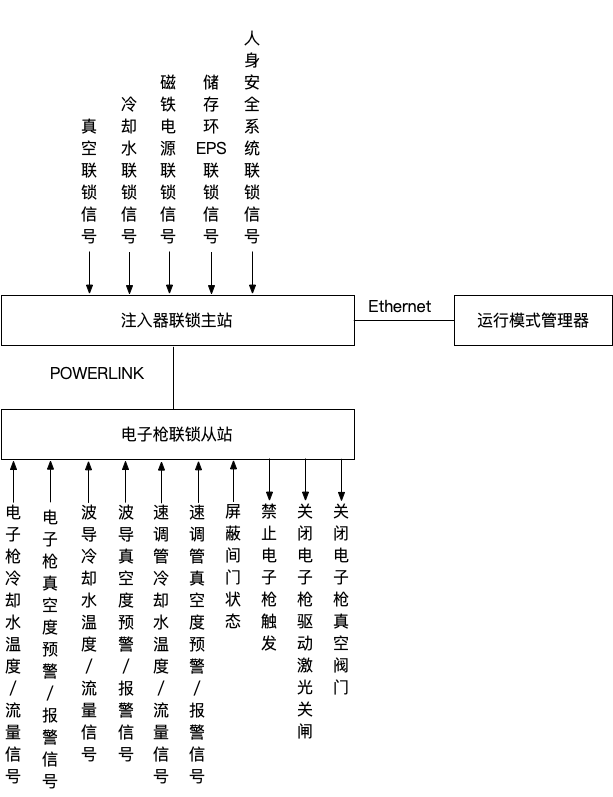
\includegraphics[width=0.5\textwidth]{linac-vacuum-eps-global.png}
	\caption{真空EPS分总体级联锁保护功能图}
	\label{fig:linac-vacuum-eps-global}
\end{figure}

\item 图~\ref{fig:linac-vacuum-eps-global}所示的真空EPS分总体级联锁保护功能,分总体级联锁输入信号包括各注入器各设备的真空计信号与真空阀门状态信号,分总体级联锁信号通过POWERLINK网络来传入POWERLINK主站,经过主站的联锁逻辑处理后,通过定时触发控制器来切断电子枪、调制器、固态放大器的同步触发信号。具体的联锁输入信号和禁止触发信号的对应关系如图~\ref{fig:linac-vacuum-eps-global}所示的虚线部分。

\end{enumerate}

\subsection{磁铁及磁铁电源EPS}
直线加速器的磁铁系统中只有聚焦磁铁线圈需要冷却,磁铁及磁铁电源EPS主要针对聚焦磁铁线圈的冷却水状态信号和磁铁电源状态信号提供保护。一般的聚焦磁铁的联锁输入信号仅会引起系统级联锁保护,速调管聚焦磁铁线圈的联锁除了系统级联锁,还会引起分总体联锁保护,具体的联锁功能归纳如下:

\begin{enumerate}
  \item 图~\ref{fig:linac-magnet-eps-system}所示的系统级联锁功能图,系统级联锁功能由磁铁及磁铁电源EPS控制器直接负责,系统联锁信号包括聚焦磁铁线圈的冷却水流量和冷却水温度信号,联锁信号直接连接到磁铁及磁铁电源EPS控制器中,控制器根据联锁逻辑,做出停止电源功率输出的动作。

  \begin{figure}[!htb]
	\centering
	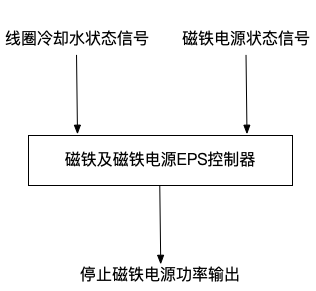
\includegraphics[width=0.4\textwidth]{linac-magnet-eps-system.png}
	\caption{磁铁及磁铁电源EPS系统级联锁功能图}
	\label{fig:linac-magnet-eps-system}
\end{figure}

  \item 图~\ref{fig:linac-magnet-eps-global}所示的速调管聚焦磁铁状态信号引起的分总体级别联锁,联锁输入信号包括磁铁电源状态信号和聚焦磁铁线圈冷却水流量温度信号。联锁信号会产生两路保护,两路保护同时发生,互为冗余。第一路是作为调制器的高压联锁信号直接输入到调制器系统,停止调制器的功率馈入;第二路是联锁信号通过POWERLINK网络来传入POWERLINK主站,经过主站的联锁逻辑处理后,通过定时触发控制器来切断调制器的同步触发信号。

  \begin{figure}[!htb]
	\centering
	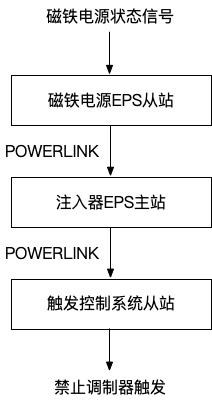
\includegraphics[width=0.65\textwidth]{linac-magnet-eps-global.png}
	\caption{磁铁及磁铁电源EPS分总体级联锁功能图}
	\label{fig:linac-magnet-eps-global}
\end{figure}
\end{enumerate}


\subsection{微波EPS}
微波系统包括速调管、加速管、聚束器等重要设备,微波EPS的功能是当微波设备发生故障或收到来自外部系统的联锁信号时,通过直接禁止调制器功率输出和禁止调制器触发的双重途径,来保护微波设备和人身安全。微波EPS的联锁输入信号主要是指各微波设备的真空状态信号和冷却水状态信号,微波EPS包括系统级联锁、分总体级联锁和总体级联锁,具体的联锁功能归纳如下:

 \begin{figure}[!htb]
	\centering
	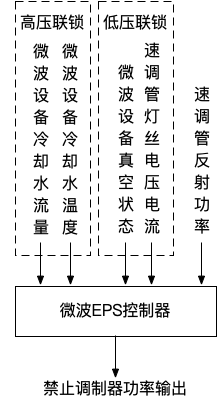
\includegraphics[width=0.3\textwidth]{linac-MW-eps-system.png}
	\caption{微波EPS系统级联锁功能图}
	\label{fig:linac-MW-eps-system}
\end{figure}

\begin{enumerate}
  \item 图~\ref{fig:linac-MW-eps-system}所示的系统级联锁功能图,系统级联锁功能由微波EPS控制器直接负责。联锁输入信号分为调制器高压联锁输入信号、调制器低压联锁输入信号和速调管反射功率信号,其中高压联锁信号包括速调管聚焦线圈的电源状态信号、各微波设备的冷却水温度流量信号,低压联锁信号包括各微波设备的真空度信号和速调管灯丝电压电流信号。联锁信号直接接入微波EPS控制器,调制器根据联锁逻辑,做出禁止调制器功率输出的保护动作。

\begin{figure}[!htb]
	\centering
	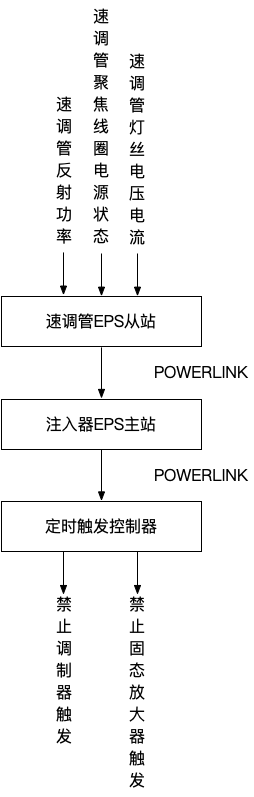
\includegraphics[width=0.5\textwidth]{linac-MW-eps-global.png}
	\caption{微波EPS分总体级和总体级联锁功能图}
	\label{fig:linac-MW-eps-global}
\end{figure}

  \item 图~\ref{fig:linac-MW-eps-global}所示的分总体级和总体级联锁功能图,分总体级联锁输入信号包括微波系统设备的全部联锁信号,总体级联锁信号是来自人身安全系统等外部系统的联锁信号,分总体级联锁信号通过POWERLINK网络来传入POWERLINK主站,经过主站的联锁逻辑处理后,通过定时触发控制器来切断调制器和固态放大器的同步触发信号。

\end{enumerate}

\subsection{冷却水联锁保护系统}
注入器存在多种不同温度的恒温冷却水系统,分别用于冷却波导管、加速管、聚束器、次谐波聚束器、速调管聚焦线圈、调制器等重要设备。图~\ref{fig:cooling-water-system-arch}是恒温冷却水系统结构图,恒温冷却水系统由去离子水站、工 艺水泵、冷却塔、板式交换机、电加热器、电动三通阀及PID控制系统组成。实现恒温控制的核心设备是PID控制器,PID控制器监测着冷却水的实时温度,当冷去水温度出现波动时,PID控制器通过预置的PID参数控制电动三通阀门开度,从而保持水温恒定。

  \begin{figure}[!htb]
	\centering
	
\includegraphics[width=0.85\textwidth]{cooling-water-system-arch.png}
	\caption{恒温冷却水系统示意图}
	\label{fig:cooling-water-system-arch}
\end{figure}

恒温冷却水系统主要负责监控各系统设备的冷却水温度和流量,为EPS提供联锁输入信号。例如,注入器每台速调管的聚焦线圈都需要进行水冷,我们将冷却水控制器采集的冷却水温度和流量信号作为微波EPS的联锁输入信号,微波EPS根据聚焦线圈的冷却水温度和流量信号的变化,提供相应保护。

\subsection{外部系统联锁信号}

\begin{figure}[!htb]
	\centering
	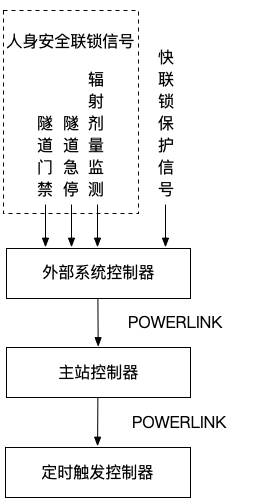
\includegraphics[width=0.333\textwidth]{outside-eps-system.png}
	\caption{外部系统联锁功能图}
	\label{fig:outside-eps-system}
\end{figure}

外部系统联锁信号属于总体级别的联锁信号,包括来自人身安全系统、快联锁保护系统、消防系统、中控急停按钮的联锁信号。图~\ref{fig:outside-eps-system}所示的外部系统联锁功能图,外部系统的联锁信号统一经由主站控制器联锁逻辑处理后,通过定时触发控制器来切断电子枪、调制器和固态放大器的同步触发信号来完成保护,具体如下:

\begin{enumerate}
  \item 人身安全系统的联锁信号包括门禁信号、隧道急停信号和辐射剂量信号等,人身安全系统控制器在综合与人身安全相关的联锁保护信号后,通过POWERLINK网络输出1路人身安全综合联锁信号到POWERLINK主站,经过主站控制器联锁逻辑处理后,通过定时触发控制器来切断电子枪、调制器和固态放大器的同步触发信号来切断束流,完成人身保护。

  \item 快联锁保护系统监测到束流偏移信号时,需要EPS提供切断束流的冗余保护。快联锁保护系统的故障信号来自束测系统,束测系统会将束流偏移信号通过POWERLINK网络输出到POWERLINK主站,经过主站控制器联锁逻辑处理后,通过定时触发控制器来切断电子枪、调制器和固态放大器的同步触发信号来切断束流。
\end{enumerate}

\subsection{定时触发控制系统}

\begin{figure}[!htb]
	\centering
	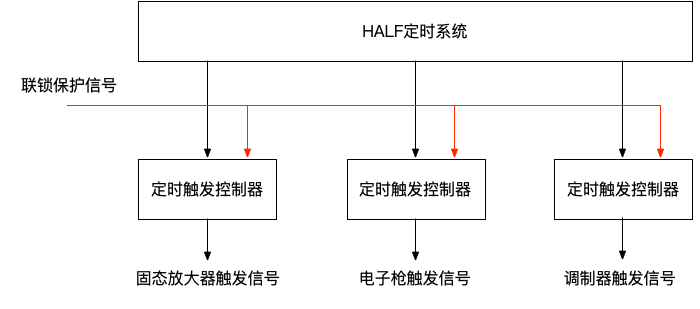
\includegraphics[width=\textwidth]{timing-control-system-eps.png}
	\caption{定时触发控制系统功能图}
	\label{fig:timing-control-system-eps}
\end{figure}

注入器EPS的联锁保护功能,主要通过定时触发控制器切断设备的同步触发信号的方式来实施。定时触发控制系统的结构如图~\ref{fig:timing-control-system-eps}所示,我们在HALF定时系统和各设备系统间设置了定时触发控制器,EPS通过定时触发控制器来切断各设备的同步触发信号。注入器EPS涉及到电子枪触发、固态放大器触发、调制器触发三路触发信号。

\subsection{输运线EPS}
束流输运线是加速器的重要组成部分,负责将直线加速器产生的束流传输到储存环注入点,储存环注入系统用于将输运到输运线末端的电子束注入到储存环中。HALF束流输运线长度为140米,输运线系统主要由冲击磁铁、切割磁铁、二极磁铁、四极磁铁、校正磁铁组成,磁铁均采用水冷却的方式,输运线的束测系统分别由若干个探测器、束流截面探测器、束流流强探测器组成。

\begin{figure}[!htb]
	\centering
	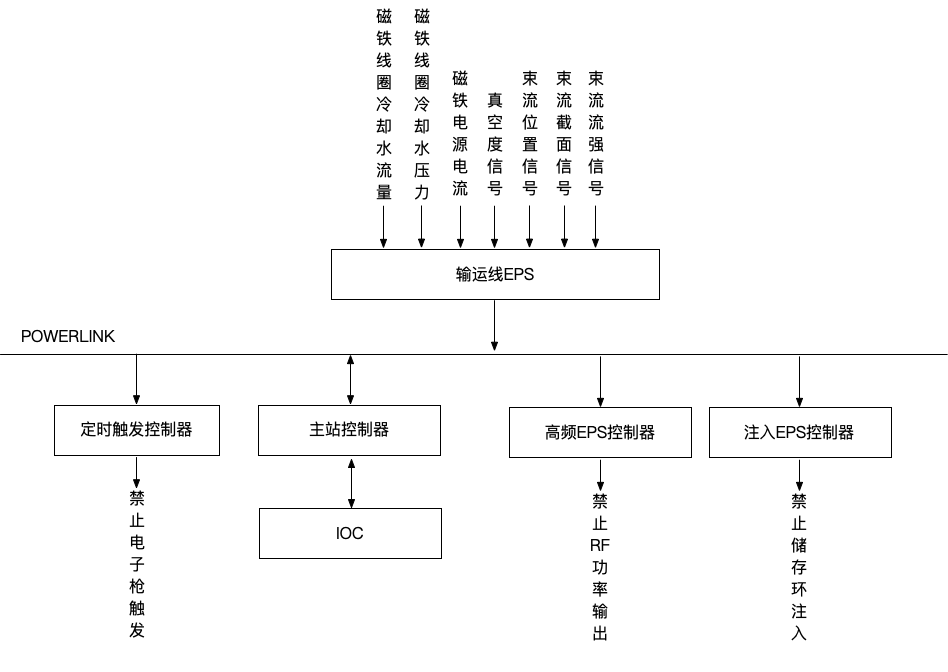
\includegraphics[width=\textwidth]{linac-eps-transportline.png}
	\caption{输运线EPS联锁功能图}
	\label{fig:linac-eps-transportline}
\end{figure}

输运线EPS的任务是当输运线范围的重要设备出现故障时,输运线EPS发出切断束流的联锁保护信号给到储存环高频系统、储存环注入系统、电子枪系统,各系统采取相应的措施停掉束流以保护设备。输运线EPS的联锁功能如图~\ref{fig:linac-eps-transportline}所示。

输运线EPS的联锁信号具体如下:
\begin{enumerate}
  \item 二极磁铁、四级磁铁、校正磁铁电源的电流信号;

  \item 二极磁铁、四级磁铁的冷却水压力和流量信号;

  \item 冲击磁铁和切割磁铁电源的电流信号;

  \item 束测状态信号,包括束流位置信号、束流截面信号、束流流强信号;

  \item 输运线的真空度信号。
\end{enumerate}

当输运线EPS的联锁信号出现异常时,会触发分总体和总体级别的保护措施,储存环高频EPS会实施禁止RF功率输出的措施,储存环注入EPS会实施禁止束流注入的措施,直线加速器EPS会实施禁止电子枪触发信号的措施。

\subsection{注入器EPS联锁逻辑总结}

注入器EPS的联锁逻辑关系如图~\ref{fig:linac-eps-table1}所示。

\begin{figure}[!htb]
	\centering
	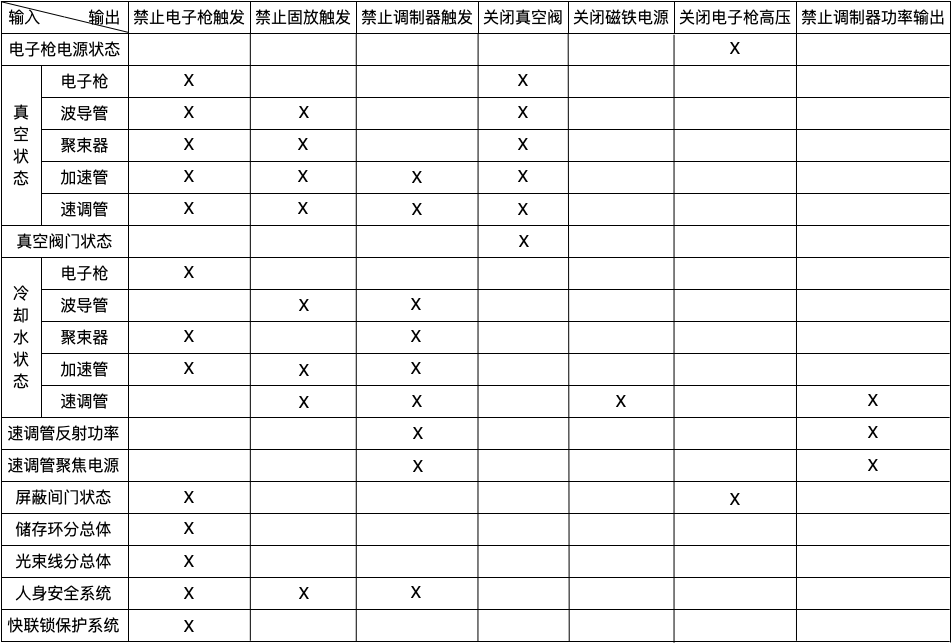
\includegraphics[width=1.1\textwidth]{linac-eps-table1.png}
	\caption{注入器EPS联锁逻辑汇总}
	\label{fig:linac-eps-table1}
\end{figure}

\begin{table}[hbt]
  \centering
  \caption{注入器EPS的联锁信号数量统计表}
  \label{table:4.2} 
  \begin{center}
  \begin{tabular}{cccccc}
    \toprule

     系统名称&联锁输入信号&联锁保护信号\\
    \midrule
    电子枪系统& 2& 2 \\
    
    真空系统  & 80 & 2 \\
    
    磁铁及磁铁电源系统 &15 & 15\\
    
    微波系统 &6  &2 \\
    
    冷却水系统  &200& 0\\

    输运线系统& 20& 0\\
    
    定时触发控制系统 &0 & 5\\
    
    人身安全系统& 1& 5\\

    快联锁保护系统&1& 5\\

    总计&325& 34\\

    \bottomrule
  \end{tabular}
\end{center}
\end{table}

根据HALF注入器的最新设计参数,注入器的联锁信号数量统计表如表~\ref{table:4.2}。

\section{储存环EPS设计}

储存环是HALF的核心部分,HALF储存环运行能量为2.2Gev,周长为480米,由磁铁、电源、真空、高频、注入、冷却水、插入件、束流测量等系统组成。储存环EPS的任务是当储存环分总体内部设备出现故障信号或者接收到来自分总体外部的联锁故障信号时,在储存环范围内及时实施相应的设备保护措施,具体的保护任务如下:

\begin{enumerate}
  \item 为储存环中各类设备提供热保护,防止设备因温度过高而损坏,保护设备主要包括:真空盒、光子吸收器、波纹管等。储存环EPS联锁输入的信号包括设备温度和设备冷却水流量与温度信号,一旦这些温度信号超过设定阈值,储存环EPS会给出禁止RF功率输出、禁止储存环注入、禁止电子枪触发等联锁保护信号。

  \item 避免储存环中设备被同步辐射光打坏,具体提供以下2种保护:\\
  1.配合快联锁保护系统完成设备快保护,保护场合是储存环电子束流偏离轨道时而导致同步辐射光直接打到真空盒、插入件、光子吸收器等重要设备,造成设备损坏;\\
  2.磁铁电源状态联锁保护,保护场合是因磁铁电源电流异常而导致电子束流偏离轨道,同步辐射光打到真空盒、插入件、光子吸收器等重要设备,造成设备损坏。

  \item 储存环的真空度联锁保护,当储存环真空度下降超过一定阈值时,储存环EPS会给出禁止RF功率输出、禁止储存环注入、禁止电子枪触发等联锁保护信号。

  \item 储存环注入系统联锁保护,保护对象是注入磁铁与电源,同时接收来自其他系统的联锁故障信号,实施禁止储存环注入的联锁保护。

  \item 插入件联锁保护,保护对象是插入件真空室及其对应的光束线真空设备,同时给束流测量系统提供插入件状态信号,配合完成快联锁保护和储存环真空度联锁保护。
\end{enumerate}

储存环EPS的联锁保护功能如图~\ref{fig:ring-interlock-signal}所示

\begin{figure}[!htb]
	\centering
	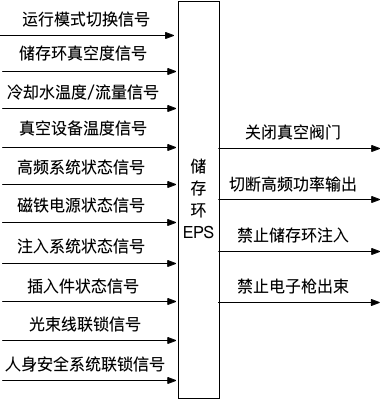
\includegraphics[width=0.7\textwidth]{ring-interlock-signal.png}
	\caption{储存环EPS联锁功能图}
	\label{fig:ring-interlock-signal}
\end{figure}

根据储存环EPS提供的联锁保护功能,我们将储存环EPS分成储存环真空EPS、磁铁及磁铁电源EPS、储存环注入EPS、插入件EPS,各系统EPS除了保证系统内设备的安全,同时需要配合快联锁保护系统等外部联锁系统的保护工作,共同完成HALF EPS的保护任务。

储存环EPS的基于POWERLINK网络和Zynq控制器来设计,储存环EPS由储存环分总体下各系统EPS组成,每个系统EPS至少由有一个控制器负责,各系统EPS控制器负责本系统内系统级的联锁保护,同时还需要将系统内的联锁信号上传至POWERLINK主站,经过联锁逻辑处理后,实施分总体级和总体级的联锁保护,同时主站控制器要将各系统设备故障数据上传至IOC,在中控系统平台上对故障数据进行存档和分析。储存环EPS各等级的联锁保护实现方式具体如下:

\begin{enumerate}
  \item 各系统EPS控制器监测本系统内部的设备状态信号,经过控制器内置的联锁保护逻辑处理后,直接实施保护动作,这种属于系统级别的保护。
  \item POWERLINK主站接收储存环分总体各系统的联锁信号,经过主站控制器的联锁保护逻辑处理后,实施禁止RF功率输出、禁止储存环注入和禁止电子枪触发信号的保护动作,这种属于分总体级别的保护。
  \item POWERLINK主站接收来自其他分总体或者外部系统的联锁信号,经过主站控制器的联锁逻辑处理后,实施禁止RF功率输出、禁止储存环注入和禁止电子枪触发信号的保护动作,这种属于总体级别的保护
\end{enumerate}

下面将详细介绍储存环分总体下各系统EPS的联锁保护功能。

\subsection{储存环真空EPS}

储存环真空EPS负责储存环真空设备热保护和储存环真空度保护。真空设备热保护的保护场合如下:

\begin{enumerate}
  \item 储存环束流流强超过一定阈值,启动热保护;

  \item 真空盒、光子吸收器和波纹管等真空设备外壁温度超过阈值,启动热保护;

  \item 真空设备的冷却水温度高于阈值或者冷却水流量低于阈值时,启动热保护。
\end{enumerate}

\begin{figure}[!htb]
	\centering
	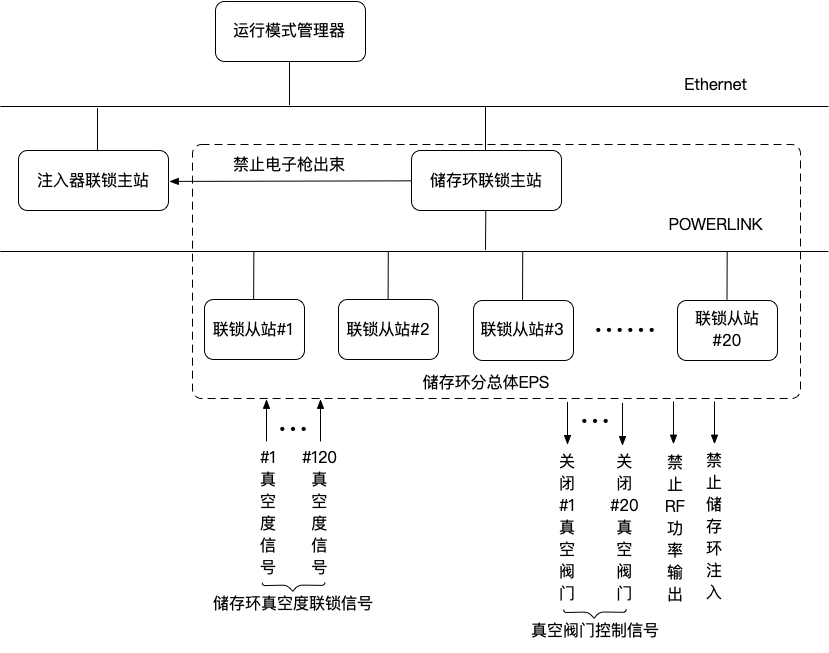
\includegraphics[width=\textwidth]{ring-eps-vacuum.png}
	\caption{真空EPS联锁功能图}
	\label{fig:ring-eps-vacuum}
\end{figure}

储存环设备热保护故障信号发生时,真空EPS会实施分总体级和总体级的保护措施,分总体级保护措施包括禁止RF功率输出以打掉束流、禁止储存环注入,总体级的保护措施为禁止电子枪触发。

真空度保护的联锁输入信号是储存环的真空度,当储存环发生真空泄漏,真空度低于阈值时,真空EPS实施分总体级和总体级的保护措施,保护措施包括禁止RF功率输出以打掉束流,禁止储存环注入,禁止电子枪触发。当束流被打掉后,真空EPS会实施关闭真空阀门的系统级保护措施。

储存环真空EPS的结构如图~\ref{fig:ring-eps-vacuum}所示。储存环真空EPS由若干个真空单元组成,每个单元需要处理的信号比较多,包括设备温度探头、冷却水流量和温度、真空度、真空阀门,这些信号的位置遍布整个储存环。储存环真空单元控制器采用Zynq控制器,每一台Zynq控制器至少负责处理一个单元的联锁信号。

\subsection{磁铁与磁铁电源EPS}

\begin{figure}[!htb]
	\centering
	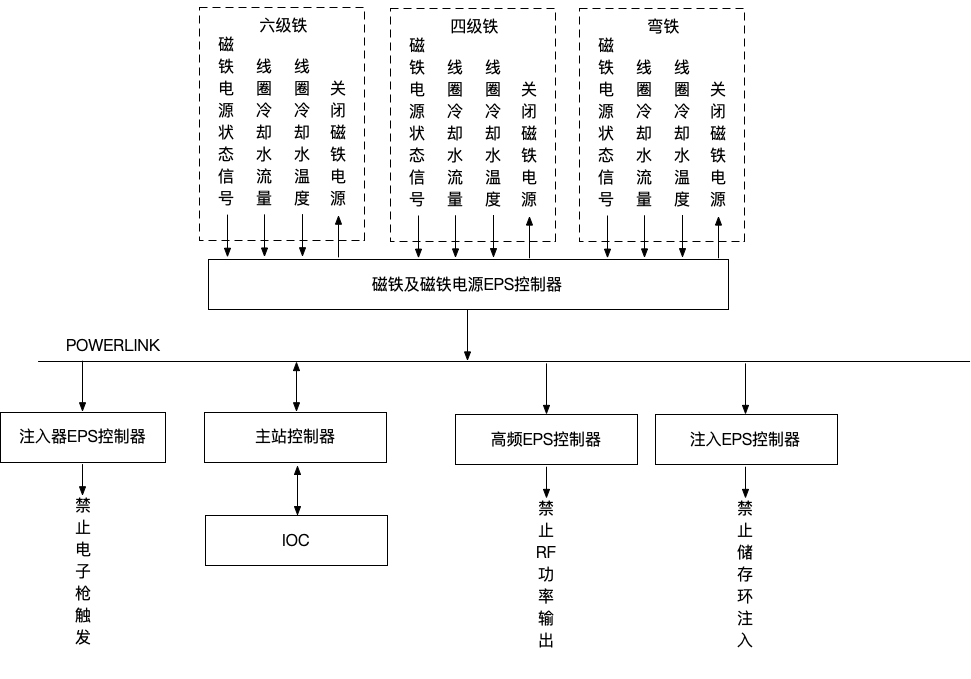
\includegraphics[width=0.9\textwidth]{ring-eps-magnet.png}
	\caption{磁铁与磁铁电源EPS联锁功能图}
	\label{fig:ring-eps-magnet}
\end{figure}

储存环中磁铁种类数量较多,有弯转二极磁铁、聚焦四极磁铁和六极磁铁。磁铁与磁铁电源EPS针对各磁铁线圈的冷却水状态信号和磁铁电源状态信号来实施相应保护措施。磁铁与磁铁电源EPS联锁功能如图~\ref{fig:ring-eps-magnet}所示,联锁输入信号会引起EPS系统级、分总体级和总体级联锁保护,具体如下:

\begin{enumerate}
  \item 系统级联锁功能由磁铁电源控制器直接负责,系统联锁输入信号包括磁铁线圈的冷却水流量、冷却水温度信号和磁铁电源状态信号,联锁输入信号直接连接到磁铁与磁铁电源EPS控制器中,控制器根据联锁逻辑,做出关闭磁铁电源的保护动作。

  \item 分总体和总体联锁信号包括磁铁电源状态信号和线圈冷却水流量温度信号,电源状态信号和线圈冷却水流量温度信号在系统EPS控制器汇总成一路联锁信号,联锁信号通过POWERLINK网络来传入POWERLINK主站,经过主站的联锁逻辑处理后,实施分总体级和总体级联锁保护。其中,分总体级联锁保护措施是通过高频EPS控制器禁止RF功率输出,通过注入系统EPS控制器停止注入;总体级联锁保护措施是通过注入器EPS禁止电子枪同步触发信号。

\end{enumerate}

\subsection{注入EPS}
储存环注入系统的任务时是把电子束流从输运线引入到储存环,注入系统的主要设备是冲击磁铁、切割磁铁及磁铁电源。注入EPS的联锁保护功能如图~\ref{fig:ring-eps-injection}所示。

\begin{figure}[!htb]
	\centering
	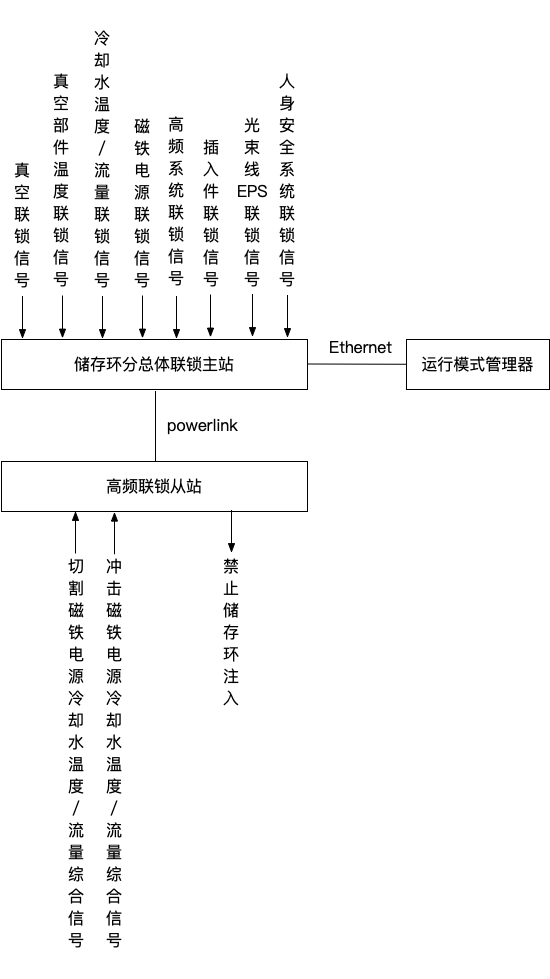
\includegraphics[width=0.9\textwidth]{ring-eps-injection.png}
	\caption{注入EPS联锁功能图}
	\label{fig:ring-eps-injection}
\end{figure}

注入EPS提供包括系统级、分总体级和总体级的联锁保护,具体如下:

\begin{enumerate}
  \item 系统级联锁功能由注入EPS控制器直接负责,系统级联锁输入信号包括冲击磁铁和切割磁铁线圈的冷却水温度流量信号、磁铁电源状态信号,联锁信号直接连接到注入EPS控制器中,当联锁输入信号出现故障时,控制器直接采取关闭磁铁电源的措施保护磁铁和电源。

  \item 注入EPS同时需要对来自储存环其他系统的联锁信号,实施禁止储存环注入的保护措施,属于分总体级别联锁保护;

  \item 注入EPS的系统级联锁输入信号还会通过POWERLINK网络来传入主站控制器,经过主站的联锁逻辑处理后,通过注入器EPS实施禁止电子枪触发的保护动作。同时高频联锁保护系统还需要接收来自快联锁保护系统和人身安全系统的联锁输入信号,实施禁止储存环注入的保护措施。
\end{enumerate}

\subsection{高频EPS}

高频系统是储存环的重要子系统,用于补充电子束流的同步辐射能量损失。一般的联锁保护动作都需要通过禁止RF功率输出来打掉束流,所以高频EPS除了需要完成系统级和分总体级的联锁保护之外,还需要接收并处理来自快联锁保护系统的束流轨道偏移信号,图~\ref{fig:ring-eps-rf}所示的高频联锁保护系统联锁功能图。

\begin{figure}[!htb]
	\centering
	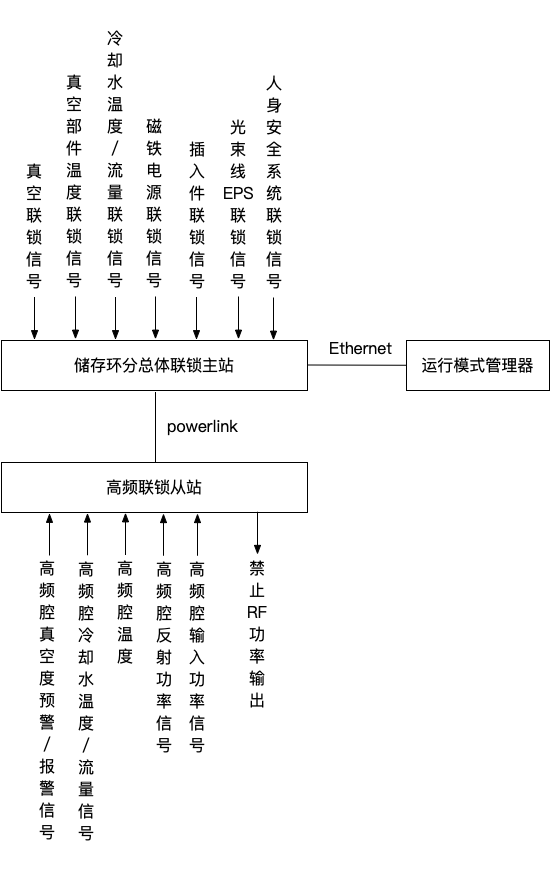
\includegraphics[width=0.9\textwidth]{ring-eps-rf.png}
	\caption{高频联锁保护系统联锁功能图}
	\label{fig:ring-eps-rf}
\end{figure}

储存环高频EPS需要提供系统级、分总体级和总体级的联锁保护,具体如下:

\begin{enumerate}
  \item 系统级联锁保护功能由高频EPS控制器直接负责,系统级联锁输入信号包括高频腔温度、冷却水流量、冷却水温度、真空度、真空阀门状态信号、RF功率信号,联锁输入信号直接连接到高频EPS控制器中,控制器根据联锁逻辑,做出关闭真空阀门、禁止RF功率输出的保护动作;

  \item 高频EPS同时需要接收来自储存环其他系统的联锁信号,实施禁止RF功率输出的设备保护动作,属于分总体级别联锁保护;

  \item 高频系统的系统级联锁输入信号还会通过POWERLINK网络来传入主站控制器,经过主站的联锁逻辑处理后,通过注入器EPS实施禁止电子枪触发的保护动作。同时高频EPS还需要接收来自快联锁保护系统的束流轨道偏移信号和人身安全系统的联锁信号,实施禁止RF功率输出的保护动作。其中快联锁保护系统的束流轨道偏移信号分成两路输入到储存环EPS中,一路直接输入到高频EPS控制器,控制器直接做出禁止RF功率的保护动作,这属于快联锁保护的范畴;另外一路通过POWERLINK传入高频EPS,然后再实施禁止RF功率输出的保护动作。两路信号互为冗余,既保证快联锁保护系统的实时性,又提高系统可靠性。
\end{enumerate}

\subsection{插入件EPS}

\begin{figure}[!htb]
	\centering
	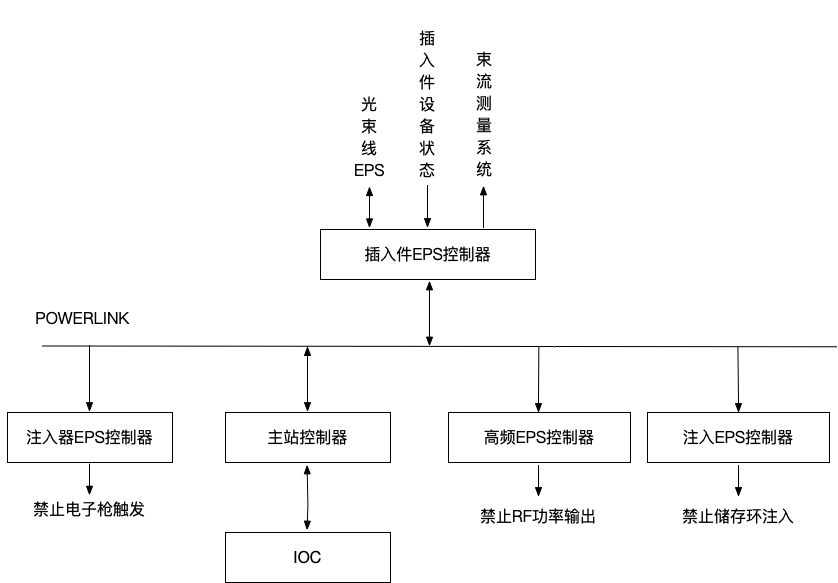
\includegraphics[width=0.9\textwidth]{ring-eps-insert.png}
	\caption{插入件EPS联锁功能图}
	\label{fig:ring-eps-insert}
\end{figure}

插入件EPS的联锁功能如图~\ref{fig:ring-eps-insert}所示,插入件EPS的任务包括提供分总体级和总体级的联锁保护,总体级联锁保护包括参与快联锁保护和光束线分总体联锁保护,分总体级联锁保护包括插入件设备故障引起的联锁保护和参与储存环真空联锁保护,具体归纳如下:

\begin{enumerate}
  \item 快联锁保护系统和储存环真空联锁保护系统的启动均与束流强度阈值有关,当束流强度超过阈值时,触发保护系统实施保护动作。束流强度阈值与是否启用插入件有关,所以插入件联锁保护系统需要将插入件状态数据发送给束测系统以确定束流强度阈值,该强度信号所对应的阈值由插入件EPS控制器给出,在束测系统内设定。

  \item 当光束线前端发生真空泄露等事故时,需要关闭真空快阀以防止真空进一步泄漏,插入件联锁保护系统必须拉开插入件间隙。

  \item 当插入件系统本身发生可能导致设备损坏的故障时,通过POWERLINK输出故障信号给主站控制器,经过主站的联锁逻辑处理后,通过高频EPS实施禁止RF功率输出的保护动作。
\end{enumerate}


\subsection{快联锁保护系统联锁信号}

\begin{figure}[!htb]
	\centering
	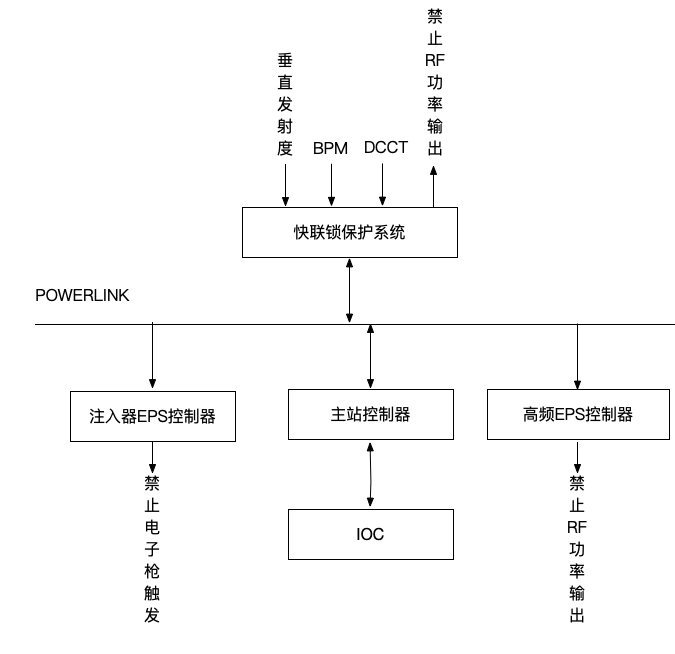
\includegraphics[width=0.9\textwidth]{ring-eps-fps.png}
	\caption{快联锁保护系统联锁功能图}
	\label{fig:ring-eps-fps}
\end{figure}


快联锁保护系统的保护场合是当束流轨道产生较大偏移时,会导致同步辐射光直接照射到真空室,强度超过一定阈值的束流会导致真空室温度过高,甚至会很快熔化真空盒,快联锁保护系统直接发出禁止RF功率输出的保护信号以打掉束流。快速联锁保护系统基于束测系统实现,直接与高频EPS相连实施保护动作。

快联锁保护系统输入信号包括束流位置信号(BPM)、束流垂直发射度和高精度直流传感器信号(DCCT),快联锁保护系统将输入信号汇总后分成两路输入到储存环EPS中,一路直接输入到高频EPS控制器,进行5$\mu$s量级的快速保护,另外一路通过POWERLINK传入高频EPS,然后再实施禁止RF功率输出的保护动作。两路保护信号互为冗余,既保证快联锁保护系统的实时性,又提高系统可靠性。

\subsection{外部系统联锁信号}

\begin{figure}[!htb]
	\centering
	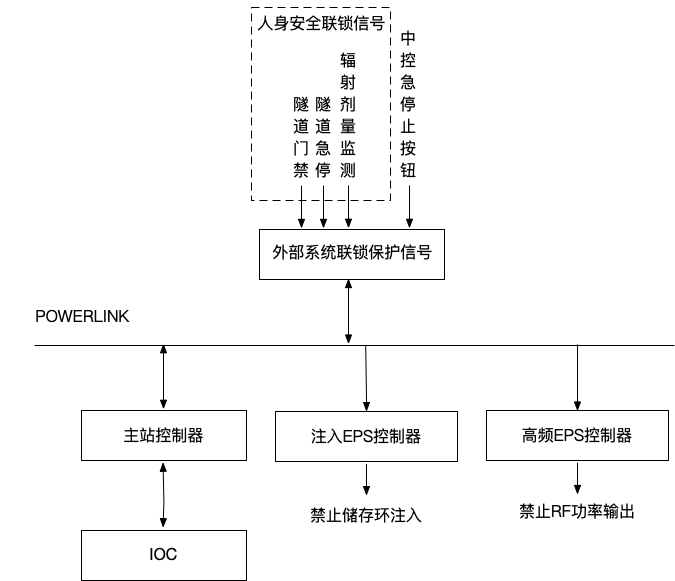
\includegraphics[width=0.9\textwidth]{ring-eps-outside.png}
	\caption{外部系统联锁功能图}
	\label{fig:ring-eps-outside}
\end{figure}

外部系统联锁信号属于总体级别的联锁信号,包括来自人身安全系统和中控急停按钮的联锁信号。图~\ref{fig:ring-eps-outside}所示的储存环外部系统联锁功能图,具体如下:

人身安全系统的联锁信号包括门禁信号、隧道急停信号和辐射剂量信号等,外部联锁控制器控制器在综合与人身安全相关的联锁保护信号后,通过POWERLINK网络输出1路人身安全综合联锁信号到POWERLINK主站,经过主站控制器联锁逻辑处理后,通过高频EPS实施禁止RF功率输出的保护动作,通过注入系统EPS实施停止注入的保护动作。

\subsection{光束线前端区EPS}

光束线分总体是HALF的重要组成部分,光束线作用是将同步辐射光从储存环引出至实验站,从而进行样品测试。HALF首期计划建设能源催化原位谱学、自旋电子材料表征、软x射线显微成像等10条光束线站。

光束线前端区是光束线与储存环连接的区域,光束线前端区EPS的任务是负责光束线前端区域的真空安全和设备安全,同时配合人身安全系统工作,保护工作人员的人身安全。光束线前端区EPS和储存环EPS之间存在着联锁保护关系,光束线前端区的设备故障会触发储存环EPS实施切断束流的保护措施。光束线前端区EPS的保护场合具体如下:

\begin{enumerate}
  \item 当光束线前端发生真空泄漏事故时,为防止真空泄漏进一步扩散,光束线前端区EPS会立即关闭真空保护快阀。由于同步辐射光的直接照射会打坏真空保护快阀,因此在真空快阀关闭前,光束线前端区EPS会切断储存环的束流,这种保护场合需要在真空泄漏信号给出后1ms内切断储存环束流。

  \item 当光束线前端区发生冷却水系统故障、束流光闸系统故障、真空阀门故障时,光束线前端区EPS通过储存环EPS实施切断束流的保护措施。

  \item 在光束线前端区束流光闸关闭前,需要发出联锁信号至对应的插入件系统要求拉开插入件间隙,然后检查插入件状态。

  \item 当光束线前端区束流光闸处于打开状态时,禁止储存环注入。

  \item 光束线前端区安全光闸只有在人身安全系统允许的情况下,才可以打开。
\end{enumerate}

\begin{figure}[!htb]
	\centering
	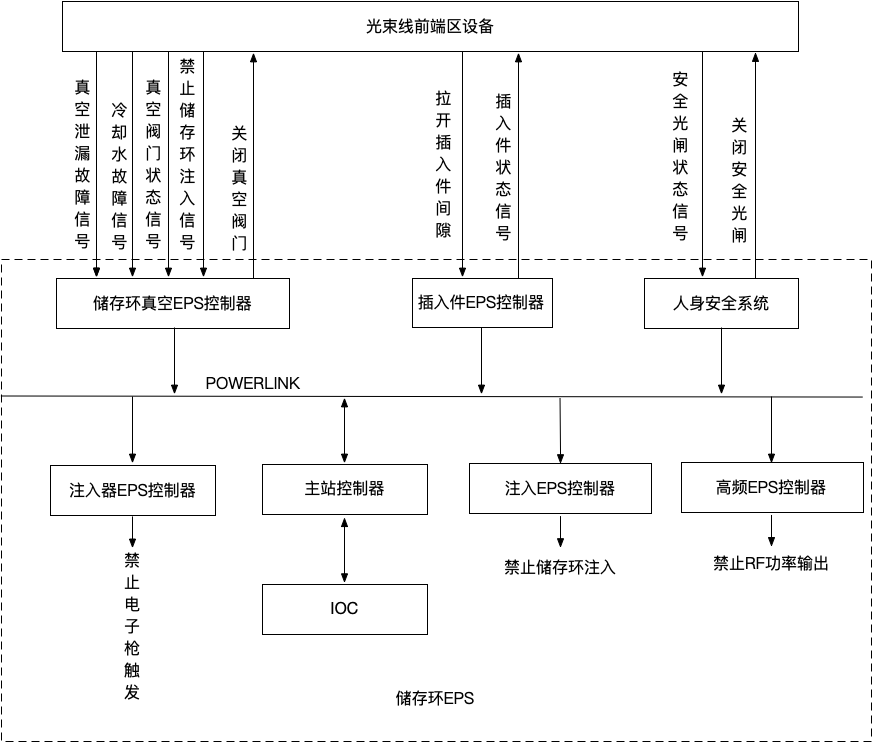
\includegraphics[width=0.9\textwidth]{light-eps.png}
	\caption{光束线前端区联锁保护系统功能图}
	\label{fig:light-eps}
\end{figure}

图~\ref{fig:light-eps}所示的为光束线前端区EPS功能图,联锁保护功能和实现方式具体如下:

\begin{enumerate}
  \item 光束线前端与储存环相衔接,采用储存环EPS的真空保护单元来处理光束线前端的联锁信号。真空单元可处理的联锁信号具体包括了光束线前端的真空度联锁信号、冷却水状态信号、真空阀门状态信号等,这些联锁故障信号会触发储存环EPS采取禁止RF功率输出、禁止电子枪触发信号、禁止储存环注入的措施来切断束流。同时对于响应时间要求在数$\mu$s量级的联锁信号,真空单元控制器会直接在本地进行快速保护,例如光束线前端出现真空泄漏时,真空单元控制器会直接采取关闭真空快阀的保护措施,同时通过高频系统禁止RF功率输出。

  \item 插入件对应光束线的联锁信号通过插入件EPS控制器来处理。在束流光闸关闭前,光束线EPS要求相应的插入件系统拉开插入件间隙,然后检查插入件系统给出插入件状态。如果插入件间隙拉开失败,则发触发储存环EPS采取禁止RF功率输出、禁止电子枪触发信号、禁止储存环注入的措施以打掉束流。

  \item 光束线前端区安全光闸的故障信号会触发人身安全系统实施相应的保护动作,同时会触发储存环EPS采取禁止RF功率输出、禁止电子枪触发信号、禁止储存环注入的措施来切断束流。


\end{enumerate}

\subsection{储存环和光束线EPS联锁逻辑总结}

储存环分总体和光束线分总体的逻辑关系如图~\ref{fig:ring-interlock}所示。

\begin{figure}[!htb]
	\centering
	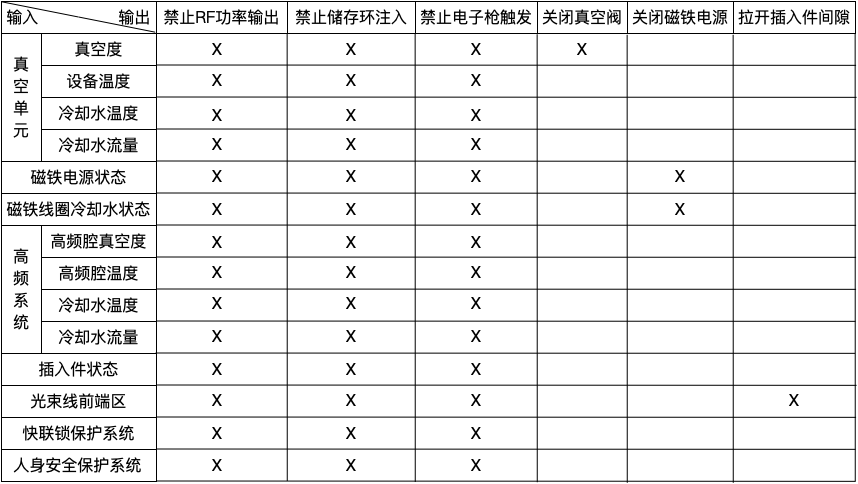
\includegraphics[width=\textwidth]{ring-interlock.png}
	\caption{储存环和光束线分总体的联锁保护逻辑图}
	\label{fig:ring-interlock}
\end{figure}

根据最新的HALF设计参数,储存环和光束线分总体的联锁信号统计如表~\ref{table:4.3}所示。
\begin{table}[hbt]
\centering
\caption{储存环和光束线EPS的联锁信号数量统计表}
\label{table:4.3} 
\begin{tabular}{|c|c|c|c|}
\hline
\multicolumn{2}{|c|}{系统}                            & \multicolumn{1}{l|}{联锁输入信号} & \multicolumn{1}{l|}{联锁输出信号} \\ \hline
\multirow{6}{*}{真空单元} & 温度信号                        & 600                         & 0                           \\ \cline{2-4} 
                      & 冷却水温度                       & 270                         & 0                           \\ \cline{2-4} 
                      & 冷却水流量                       & 280                         & 0                           \\ \cline{2-4} 
                      & 真空度                         & 130                         & 30                          \\ \cline{2-4} 
                      & \multicolumn{1}{l|}{真空阀门状态} & 30                          & 0                           \\ \cline{2-4} 
                      & 光束线                         & 195                         & 5                           \\ \hline
\multicolumn{2}{|c|}{高频系统}                          & 1                           & 3                           \\ \hline
\multicolumn{2}{|c|}{注入系统}                          & 1                           & 1                           \\ \hline
\multicolumn{2}{|c|}{插入件系统}                         & 50                          & 25                          \\ \hline
\multicolumn{2}{|c|}{磁铁及磁铁电源}                       & 50                          & 0                           \\ \hline
\multicolumn{2}{|c|}{人身安全系统}                        & 1                           & 1                           \\ \hline
\multicolumn{2}{|c|}{快联锁保护系统}                       & 1                           & 0                           \\ \hline
\multicolumn{2}{|c|}{总计}                            & 1609                        & 65                          \\ \hline
\end{tabular}
\end{table}

\section{HALF注入器设备联锁保护原型系统}

根据HALF注入器设备联锁保护系统的联锁功能和结构特点,我们设计并搭建了相应的原型系统,并进行了相关的功能测试,以下将分别介绍原型系统的系统设计、硬件组成、软件开发和性能测试。

\subsection{原型系统设计和硬件组成}

\begin{figure}[!htb]
	\centering
	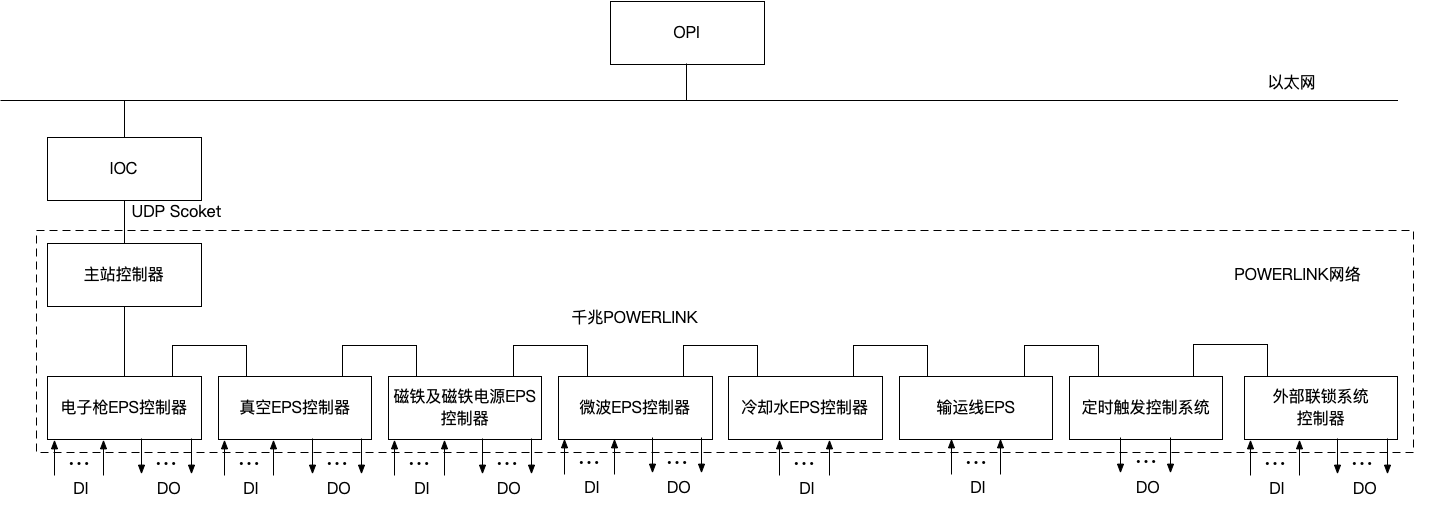
\includegraphics[width=\textwidth]{prototype-half-linac.png}
	\caption{注入器EPS原型系统结构图}
	\label{fig:prototype-half-linac}
\end{figure}

注入器EPS的原型系统架构如图~\ref{fig:prototype-half-linac}所示,注入器EPS由分总体下的各系统EPS组成,每个系统EPS的控制器是采用基于Zynq的控制器,Zynq控制器配置多路DI/DO通道,用于采集各系统内需要监测的设备状态信号和输出相应的保护动作。各系统控制器按照线型拓扑结构依次相连,各系统控制器之间基于千兆POWERLINK通信。POWERLINK主站同样采用基于Zynq的控制器,主站负责处理分总体级和总体级联锁保护逻辑,同时主站会将注入器EPS各系统的状态数据传输给IOC,并接收来自IOC的控制命令,IOC与主站控制器之间的通信基于UDP Socket来实现。操作人员通过OPI来实时监测EPS各系统内设备的安全状态,并设置一些EPS控制参数。

注入器EPS原型系统需要处理不同等级的联锁信号,具体处理方式如下:

\begin{enumerate}
  \item 系统级联锁:系统级联锁通过Zynq控制器完成。各系统内需要监测的设备状态信号直接接入到各系统控制器中,通过控制器预设的联锁逻辑处理后,输出保护动作。

  \item 分总体级和总体级联锁:分总体级和总体级联锁通过POWERLINK网络实现。系统控制器将采集到的设备状态数据通过POWERLINK网络传输给主站,主站经过联锁逻辑处理后,通过定时触发控制系统来切断相应设备的同步触发信号,从而提供保护。

\end{enumerate}

注入器EPS需要监测的各系统设备信号数量如表~\ref{table:4.2}所示,其中共有325个联锁输入信号,34个联锁输出信号。第~\ref{section:方案2系统设计与原型系统开发}节中设计的基于POWERLINK的分布式IO系统由5个从站组成,一共可以提供640个DI通道,90个DO通道,完全可以满足注入器EPS原型系统信号数量的需求。所以我们直接基于第~\ref{section:方案2系统设计与原型系统开发}节中原型系统的硬件设备进行开发,其中原型系统中的每个Zynq控制器至少负责一个注入器子系统的联锁保护,每个系统的联锁信号类型均为数字信号。

\subsection{软件开发}

原型系统的软件开发包括了Zynq控制器程序的开发、EPICS设备驱动程序的开发和OPI的开发,下面将分别介绍程序的设计和开发细节。

\subsubsection{Zynq控制器程序的开发}

Zynq控制器程序的开发包括各系统控制器程序开发和主站控制器程序开发。系统控制器的程序结构如图~\ref{fig:prototype-zynq-software}所示,控制器程序分为POWERLINK协议和系统级联锁处理算法两个部分,其中POWERLINK协议的数据链路层和物理层协议基于FPGA实现,已在第~\ref{section:方案2系统设计与原型系统开发}节中Zynq控制器软件设计部分详细介绍,在此不再赘述。如图~\ref{fig:prototype-zynq-software}所示,联锁处理算法模块“Interlock Algorithm”和信号预处理模块“Preprocess”添加在POWERINK应用层中,基于ARM实现。

设备信号首先经过“Preprocess”模块的预处理,预处理流程如图~\ref{fig:preprocess}所示,预处理模块负责对设备信号进行是否被旁路、是否被锁存、是否存活的判断,只有未被旁路、未被锁存、存活的信号才能被联锁处理算法模块处理。信号的旁路、锁存、存活状态具体解释如下:

\begin{enumerate}
  \item 旁路:在某些特殊情况下需要临时解除对个别输入信号的联锁响应,通过将输入信号设置成旁路状态来实现这种需求。旁路的原理:输入信号被设置成旁路状态后,输入信号的实时状态仍可以正常显示,但当输入信号处于报警状态时不会引起系统的联锁保护响应。

  \item 锁存:通过将输入信号设置成锁存状态,可以保持输入信号的报警状态不变。当输入信号从报警状态恢复到正常状态后,被锁存的输入信号将继续处于报警状态,输入信号引起的联锁输出信号也保持为保护状态,当操作人员解除该输入信号锁存时,才能取消信号的报警状态,从而解除联锁输出信号的保护状态。

 \item 存活:主要是指设备信号是否存在,硬件设备是否继续与控制器保持连接。

\end{enumerate}

信号的锁存状态和旁路状态是操作人员通过IOC进行设置的。联锁保护算法模块负责对经过预处理的信号进行联锁逻辑处理,并输出相应的联锁保护动作。

\begin{figure}[!htb]
	\centering
	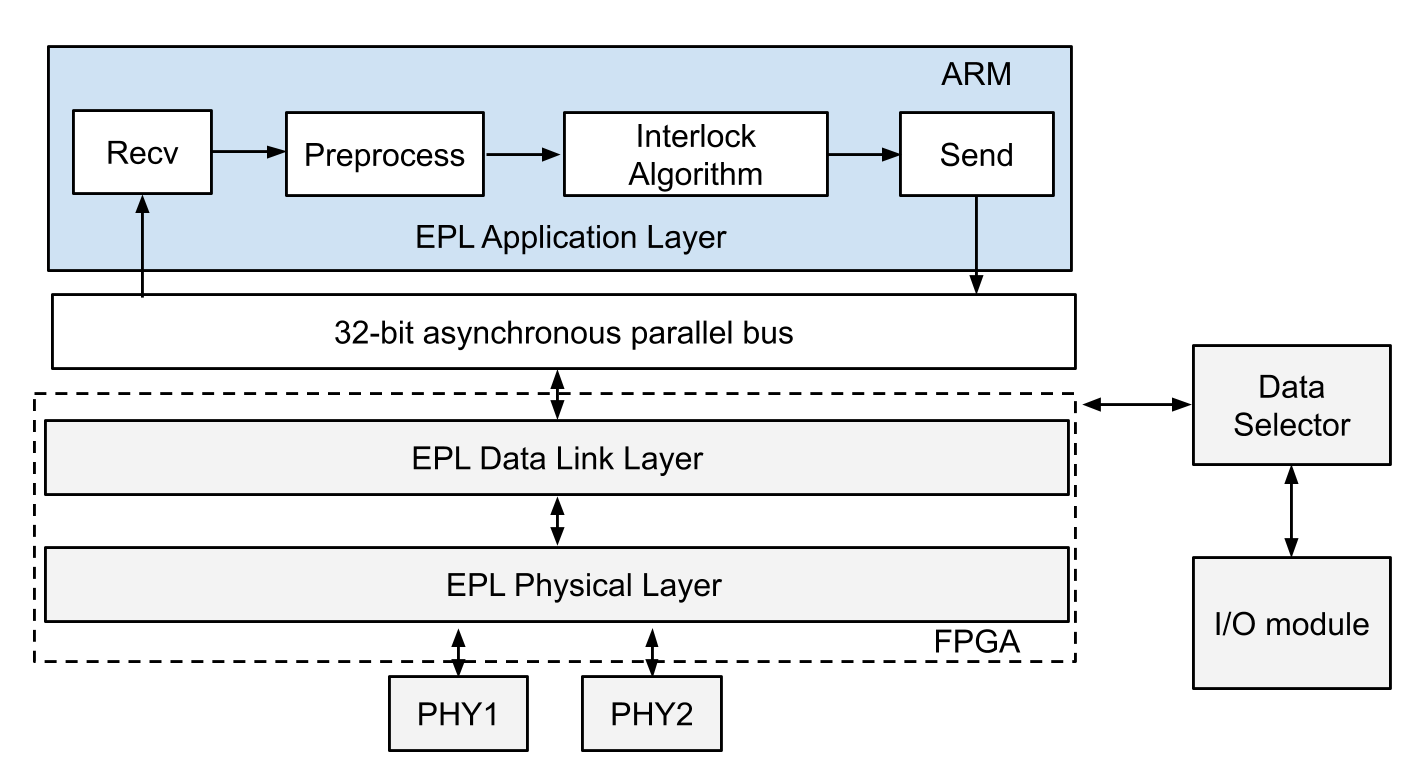
\includegraphics[width=\textwidth]{prototype-zynq-software.png}
	\caption{原型系统控制器软件结构图}
	\label{fig:prototype-zynq-software}
\end{figure}

\begin{figure}[!htb]
	\centering
	
\includegraphics[width=0.4\textwidth]{preprocess.png}
	\caption{输入信号预处理流程图}
	\label{fig:preprocess}
\end{figure}

主站控制器的软件架构如图~\ref{fig:prototype-mn-software}所示的“MN”部分,其中POWERLINK协议的数据链路层和物理层基于FPGA实现,已在第~\ref{section:方案2系统设计与原型系统开发}节中Zynq控制器软件设计部分详细介绍,在此不再赘述。分总体级和总体级的联锁处理算法模块“Interlock Algorithm”添加在POWERINK应用层中,基于ARM实现。联锁处理算法模块负责对来自注入器内各系统或者其他分总体的设备信号进行处理,然后通过定时触发控制器切断相应的同步触发信号来实施保护。除了完成联锁保护的任务,主站应用层程序还需要接收来自IOC的控制参数,控制参数主要包括对信号进行旁路、锁存、重置的设置,控制参数储存在“Output data”缓存区中,会通过POWERLINK将参数设到相应的系统控制器。同时主站程序会将各系统的设备状态数据存储在“Input Data”缓存区中,并传输到IOC,让操作人员可以通过OPI进行实时监控。

\begin{figure}[!htb]
	\centering
	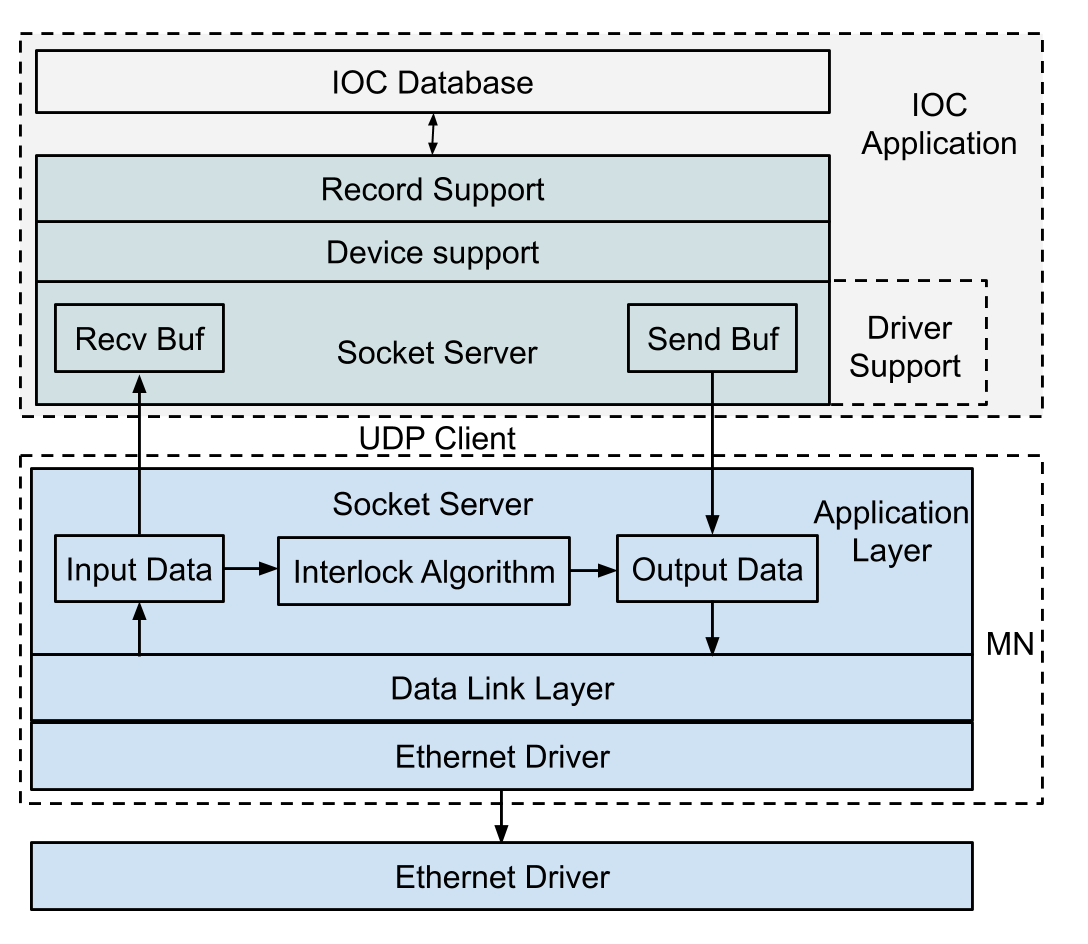
\includegraphics[width=0.6\textwidth]{prototype-mn-software.png}
	\caption{主站与IOC的软件架构}
	\label{fig:prototype-mn-software}
\end{figure}

\subsubsection{EPICS设备驱动程序的开发}
EPICS设备驱动程序的架构如图~\ref{fig:prototype-mn-software}所示,信号类型主要为数字输入和数字输出,所以可以直接采用用标准的EPICS DI和DO记录来监控设备信号。

\subsubsection{原型系统OPI的开发}

Phoebus/Display Builder是EPICS社区最新发布的OPI图形界面开发软件,Phoebus是用于对大规模控制系统进行监控和操作的一个软件框架和工具集,它是Control System Studio(CS-Studio)工具集的最新升级版本,不需要再依赖于Eclipse的RCP和SWT开发工具,也不再使用Workspace,提高了软件使用的方便性。我们采用Phoebus/Display Builder作为注入器EPS原型系统的控制界面开发工具。

原型系统的OPI和IOC运行在同一台PC上,图~\ref{fig:main-panel}所示的为注入器EPS的主界面,图中采用颜色来表示信号的状态,其中绿色表示数字信号“0”,红色表示数字信号“1”。当系统中出现设备故障信号(数字信号“1”)时,该系统图标颜色会变成深灰色,图标下的箭头会变成红色。定时触发控制系统的输出信号颜色为红色时,表示禁止相应设备的同步触发信号,绿色表示允许相应设备的同步触发信号。图~\ref{fig:main-panel}中所示的情况是某设备的真空信号处于故障状态,定时触发控制系统输出禁止电子枪和调制器的触发信号。

\begin{figure}[!htb]
	\centering
	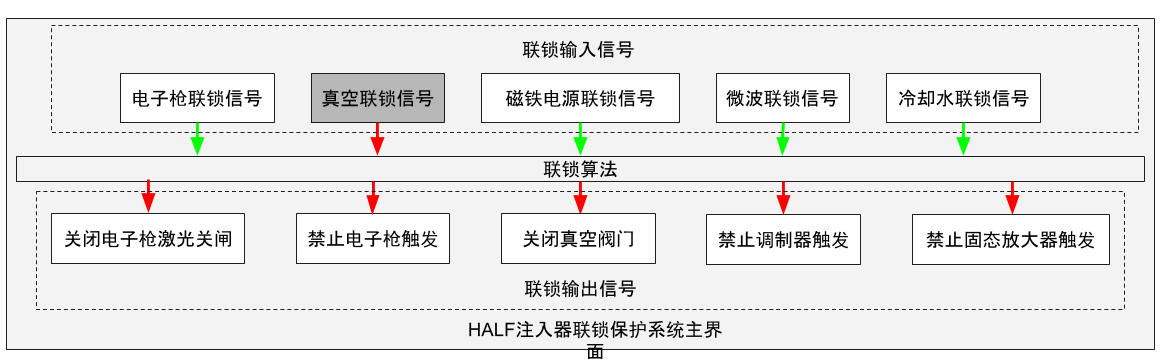
\includegraphics[width=\textwidth]{main-panel.png}
	\caption{注入器EPS的主界面}
	\label{fig:main-panel}
\end{figure}

当点击系统图标时,会弹出新界面,显示该系统的详细情况。图~\ref{fig:vacuum-panel}所示的为真空系统的详细界面,其中速调管和真空阀门图标颜色为红色,表示速调管真空状态出现故障,真空阀门处于关闭状态;其余设备图标颜色为绿色,表示真空状态正常。

\begin{figure}[!htb]
	\centering
	\includegraphics[width=\textwidth]{vacuum-panel.png}
	\caption{真空系统EPS界面}
	\label{fig:vacuum-panel}
\end{figure}

点击速调管图标后,会弹出如图~\ref{fig:k-vacuum-panel}所示的详细界面,显示每台速调管的真空状态。真空信号状态的变化由不同的颜色来表示,红色、绿色和黑色分别表示了真空信号处于报警、正常或失联状态。操作人员可以直接在面板上点击旁路、锁存或重置的图标对信号进行相应处理,图标颜色为绿色时,表示开启了相应处理,图标为灰色表示关闭了相应处理。图~\ref{fig:k-vacuum-panel}中所示的情况为,第二台速调管的真空信号(VS2)处于报警状态。

\begin{figure}[!htb]
	\centering
	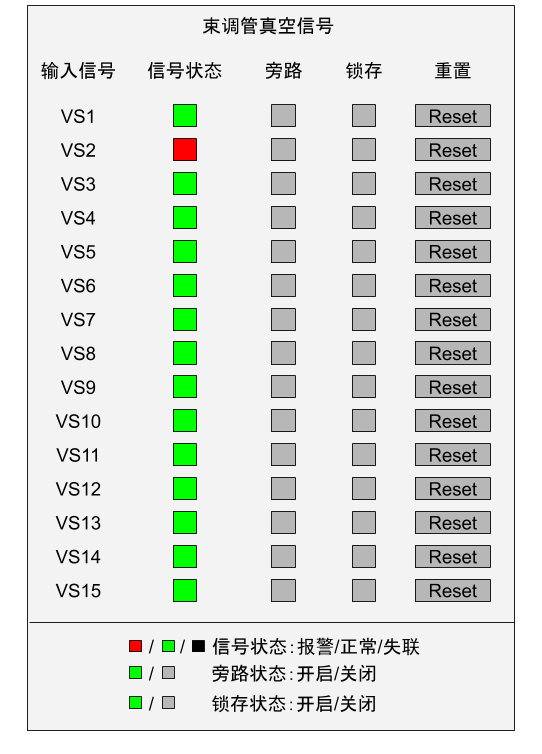
\includegraphics[width=0.6\textwidth]{k-vacuum-panel.png}
	\caption{速调管设备真空状态信号}
	\label{fig:k-vacuum-panel}
\end{figure}


\subsection{性能测试}

原型系统的POWERLINK通信周期被配置为50$\mu$s,我们对图~\ref{fig:k-vacuum-panel}和图~\ref{fig:main-panel}中的联锁保护场合进行了响应时间的测试,即速调管真空信号(VS2)处于报警状态时,会引起真空阀门关闭的系统级联锁保护动作和禁止电子枪触发信号的分总体级联锁保护动作。

真空EPS由1号从站控制器负责,我们将1号从站控制器的输入和输出信号连接到示波器上,以输入和输出信号的上升沿时间差来表示系统级响应时间。测试结果如图~\ref{fig:vacuum-off}所示,Ch2(青色线)代表速调管的真空信号,Ch3(红色线)代表真空阀的关闭信号,响应时间约为5$\mu$s。

\begin{figure}[!htb]
	\centering
	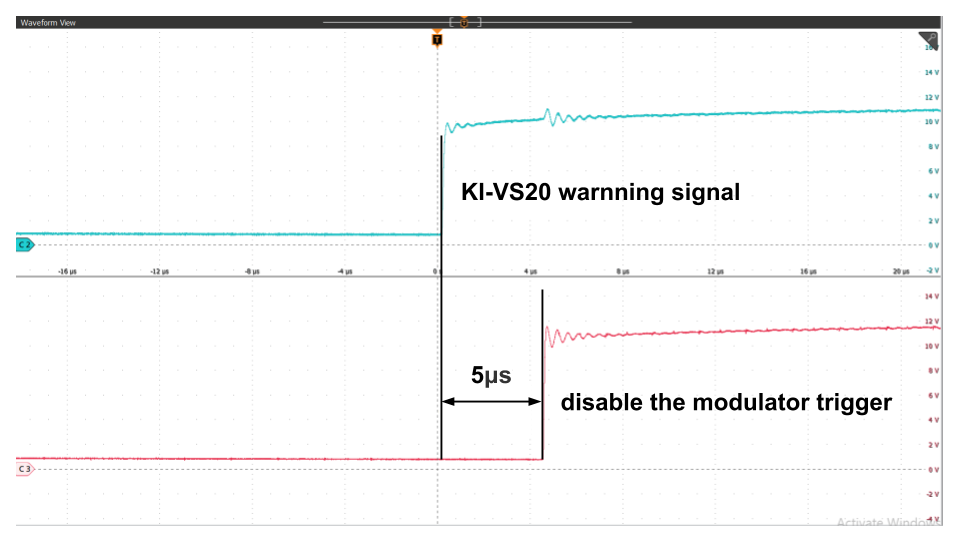
\includegraphics[width=0.8\textwidth]{vacuum-off.png}
	\caption{真空EPS系统级联锁保护时间测试结果}
	\label{fig:vacuum-off}
\end{figure}

定时触发控制系统由5号从站控制器负责,我们将1号从站控制器的输入和5号从站控制器的输出信号连接到示波器上,以输入和输出信号的上升沿时间差来表示分总体级响应时间。测试结果如图~\ref{fig:e-gun-trigger}所示, Ch2(青色线)代表速调管的真空信号; Ch1(黑线)代表禁止电子枪触发信号,响应时间约为160$\mu$s。

\begin{figure}[!htb]
	\centering
	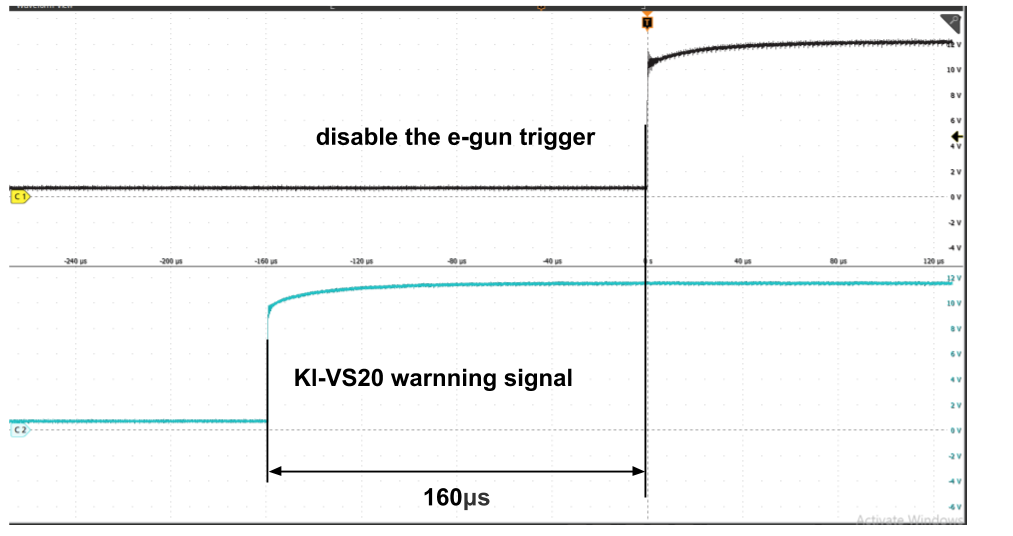
\includegraphics[width=0.8\textwidth]{e-gun-trigger.png}
	\caption{真空EPS分总体级联锁保护时间测试结果}
	\label{fig:e-gun-trigger}
\end{figure}

\subsection{注入器EPS联锁逻辑总结}

根据上述注入器EPS各系统的联锁保护功能,现将注入器EPS的联锁逻辑关系总结如表~\ref{table:4.2}所示。


% Please add the following required packages to your document preamble:
% \usepackage{multirow}
\begin{table}[!htb]
\centering\small
\caption{注入器EPS的联锁逻辑汇总表}
\label{table:4.2}
\begin{tabular}{|l|c|l|l|l|}
\hline
\multicolumn{2}{|c|}{\diagbox[width=12em,trim=l]{联锁输入}{联锁保护}}                                                              & 禁止电子枪触发 & 禁止调制器触发 & 禁止固放触发 \\ 
\hline
\multicolumn{2}{|c|}{电子枪灯丝电源}                                                                     &    \multicolumn{1}{c|}{√}     &        &        \\ \hline
\multicolumn{2}{|c|}{屏蔽间门状态}                                                                      &    \multicolumn{1}{c|}{√}      &        &        \\ \hline
\multirow{8}{*}{\begin{tabular}[c]{@{}l@{}}真\\ 空\\ 联\\ 锁\\ 信\\ 号\end{tabular}}      & 电子枪真空度      &    \multicolumn{1}{c|}{√}      &        &        \\ \cline{2-5} 
                                                                                    & 电子枪真空阀门     &    \multicolumn{1}{c|}{√}     &        &        \\ \cline{2-5} 
                                                                                    & 聚束器真空度      &     \multicolumn{1}{c|}{√}    &    \multicolumn{1}{c|}{√}     &    \multicolumn{1}{c|}{√}     \\ \cline{2-5} 
                                                                                    & 加速管真空度      &    \multicolumn{1}{c|}{√}    &    \multicolumn{1}{c|}{√}     &     \multicolumn{1}{c|}{√}   \\ \cline{2-5} 
                                                                                    & 加速管真空阀门     &    \multicolumn{1}{c|}{√}      &   \multicolumn{1}{c|}{√}     &    \multicolumn{1}{c|}{√}     \\ \cline{2-5} 
                                                                                    & 速调管真空度      &         &   \multicolumn{1}{c|}{√}     &    \multicolumn{1}{c|}{√}     \\ \cline{2-5} 
                                                                                    & 波导真空度       &         &    \multicolumn{1}{c|}{√}    &    \multicolumn{1}{c|}{√}     \\ \cline{2-5} 
                                                                                    & 输运线真空度      &   \multicolumn{1}{c|}{√}       &        &        \\ \hline
\multicolumn{2}{|c|}{磁铁电源状态}                                                                      &    \multicolumn{1}{c|}{√}     &   \multicolumn{1}{c|}{√}      &    \multicolumn{1}{c|}{√}     \\ \hline
\multicolumn{2}{|c|}{速调管聚焦线圈电源}                                                                   &         &    \multicolumn{1}{c|}{√}     &    \multicolumn{1}{c|}{√}     \\ \hline
\multicolumn{2}{|c|}{速调管反射功率}                                                                     &         &   \multicolumn{1}{c|}{√}      &    \multicolumn{1}{c|}{√}     \\ \hline
\multicolumn{2}{|c|}{速调管灯丝电压电流}                                                                   &         &    \multicolumn{1}{c|}{√}     &    \multicolumn{1}{c|}{√}     \\ \hline
\multicolumn{2}{|c|}{调制器状态}                                                                      &         &   \multicolumn{1}{c|}{√}      &   \multicolumn{1}{c|}{√}      \\ \hline
\multirow{12}{*}{\begin{tabular}[c]{@{}l@{}}冷\\ 却\\ 水\\ 联\\ 锁\\ 信\\ 号\end{tabular}} & 磁铁线圈冷却水温度   &  \multicolumn{1}{c|}{√}        &   \multicolumn{1}{c|}{√}      &    \multicolumn{1}{c|}{√}     \\ \cline{2-5} 
                                                                                    & 磁铁线圈冷却水流量   &    \multicolumn{1}{c|}{√}      &   \multicolumn{1}{c|}{√}      &   \multicolumn{1}{c|}{√}      \\ \cline{2-5} 
                                                                                    & 聚束器冷却水温度    &    \multicolumn{1}{c|}{√}      &   \multicolumn{1}{c|}{√}      &    \multicolumn{1}{c|}{√}     \\ \cline{2-5} 
                                                                                    & 聚束器冷却水流量    &    \multicolumn{1}{c|}{√}      &   \multicolumn{1}{c|}{√}      &    \multicolumn{1}{c|}{√}     \\ \cline{2-5} 
                                                                                    & 加速管冷却水温度    &  \multicolumn{1}{c|}{√}        &  \multicolumn{1}{c|}{√}       &    \multicolumn{1}{c|}{√}     \\ \cline{2-5} 
                                                                                    & 加速管冷却水流量    &    \multicolumn{1}{c|}{√}      &   \multicolumn{1}{c|}{√}      &   \multicolumn{1}{c|}{√}      \\ \cline{2-5} 
                                                                                    & 速调管管体冷却水温度  &          &   \multicolumn{1}{c|}{√}      &    \multicolumn{1}{c|}{√}     \\ \cline{2-5} 
                                                                                    & 速调管管体冷却水流量  &          &   \multicolumn{1}{c|}{√}      &   \multicolumn{1}{c|}{√}      \\ \cline{2-5} 
                                                                                    & 速调管输出窗冷却水温度 &          &   \multicolumn{1}{c|}{√}      &    \multicolumn{1}{c|}{√}     \\ \cline{2-5} 
                                                                                    & 速调管输出窗冷却水流量 &          &   \multicolumn{1}{c|}{√}      &   \multicolumn{1}{c|}{√}      \\ \cline{2-5} 
                                                                                    & 波导冷却水温度     &          &  \multicolumn{1}{c|}{√}       &   \multicolumn{1}{c|}{√}      \\ \cline{2-5} 
                                                                                    & 波导冷却水流量     &          &   \multicolumn{1}{c|}{√}      &   \multicolumn{1}{c|}{√}      \\ \hline
\multicolumn{2}{|c|}{储存环分总体EPS联锁信号}                                                               &   \multicolumn{1}{c|}{√}       &        &        \\ \hline
\multicolumn{2}{|c|}{人身安全系统联锁信号}                                                                  &   \multicolumn{1}{c|}{√}       &        &        \\ \hline
\multicolumn{2}{|c|}{光束线联锁信号}                                                                     &  \multicolumn{1}{c|}{√}        &        &        \\ \hline
\end{tabular}
\end{table}

% Please add the following required packages to your document preamble:
% \usepackage{multirow}
\begin{table}[]
\centering\small
\begin{tabular}{|l|c|l|l|l|l|l|}
\hline
\multicolumn{2}{|l|}{}                                                                   & 禁止电子枪触发                & 禁止固放触发                 & 禁止固放触发                 & \multicolumn{1}{c|}{关闭激光关闸} & \multicolumn{1}{c|}{关闭真空阀门} \\ \hline
\multicolumn{2}{|c|}{电子枪灯丝电源}                                                            & \multicolumn{1}{c|}{√} & \multicolumn{1}{c|}{√} & \multicolumn{1}{c|}{√} &                             &                             \\ \hline
\multicolumn{2}{|c|}{屏蔽间门状态}                                                             &                        &                        &                        &                             &                             \\ \hline
\multirow{8}{*}{\begin{tabular}[c]{@{}l@{}}真\\ 空\\ 联\\ 锁\\ 信\\ 号\end{tabular}} & 电子枪真空度  & \multicolumn{1}{c|}{√} &                        &                        &                             &                             \\ \cline{2-7} 
                                                                               & 电子枪真空阀门 &                        &                        &                        &                             &                             \\ \cline{2-7} 
                                                                               & 聚束器真空度  &                        &                        &                        &                             &                             \\ \cline{2-7} 
                                                                               & 加速管真空度  &                        &                        &                        &                             &                             \\ \cline{2-7} 
                                                                               & 加速管真空阀门 &                        &                        &                        &                             &                             \\ \cline{2-7} 
                                                                               & 速调管真空度  &                        &                        &                        &                             &                             \\ \cline{2-7} 
                                                                               & 波导真空度   &                        &                        &                        &                             &                             \\ \cline{2-7} 
                                                                               & 输运线真空度  &                        &                        &                        &                             &                             \\ \hline
\multicolumn{2}{|c|}{磁铁电源状态}                                                             &                        &                        &                        &                             &                             \\ \hline
\multicolumn{2}{|c|}{速调管聚焦线圈电源}                                                          &                        &                        &                        &                             &                             \\ \hline
\multicolumn{2}{|c|}{速调管反射功率}                                                            &                        &                        &                        &                             &                             \\ \hline
\multicolumn{2}{|c|}{速调管灯丝电压电流}                                                          &                        &                        &                        &                             &                             \\ \hline
\end{tabular}
\end{table}

根据HALF注入器的最新设计参数,注入器的联锁信号数量统计表如表~\ref{table:4.3}。

\begin{table}[!hbt]
  \centering
  \caption{注入器EPS的联锁信号数量统计表}
  \label{table:4.3} 
  \begin{center}
  \begin{tabular}{cccccc}
    \toprule

     系统名称&联锁输入信号&联锁保护信号\\
    \midrule
    电子枪系统& 2& 0 \\
    
    真空系统  & 65 & 0 \\
    
    磁铁电源系统 &15 & 0\\
    
    微波系统 &60  &0 \\
    
    冷却水系统  &192& 0\\

    调制器系统& 1& 0\\
    
    定时触发控制系统 &0 & 3\\

    储存环分总体EPS & 1& 0\\
    
    人身安全系统& 1& 0\\

    快联锁保护系统&1& 0\\

    总计&338& 3\\

    \bottomrule
  \end{tabular}
\end{center}
\end{table}

\section{储存环EPS设计}

储存环是HALF的核心部分,HALF储存环采用衍射极限储存环的方案,运行能量为2.2Gev,周长为480米。输运线中的电子束流经过注入系统传输到储存环中,储存环中的电子束在磁场作用下沿着束流轨道做回旋运动,在储存环的切线方向上释放出同步辐射光。储存环有多个直线节,分别用于储存环注入系统的安装,把注入器的束流注入到储存环中;用于高频系统的安装,用于补充电子束流饮释放同步辐射光损失的能量;用于根据同步辐射实验需求安装不同类型的插入元件,同时支持多个用户的同步辐射实验研究。

HALF由磁铁、电源、真空、高频、注入、冷却水、插入件、束流测量等系统组成。

HAL储存环分总体由真空系统、冷却水系统、磁铁及磁铁电源系统、高频系统、插入件、冷却水系统、束流测量系统等组成,注入器的主要设备包括电子枪、聚束器、加速管、聚焦磁铁组、固态放大器、速调管、调制器和束测设备。




储存环EPS的任务是当储存环分总体内部设备出现故障信号或者接收到来自分总体外部的联锁故障信号时,在储存环范围内及时实施相应的设备保护措施,具体的保护任务如下:

\begin{enumerate}
  \item 为储存环中各类设备提供热保护,防止设备因温度过高而损坏,保护设备主要包括:真空盒、光子吸收器、波纹管等。储存环EPS联锁输入的信号包括设备温度和设备冷却水流量与温度信号,一旦这些温度信号超过设定阈值,储存环EPS会给出禁止RF功率输出、禁止储存环注入、禁止电子枪触发等联锁保护信号。

  \item 避免储存环中设备被同步辐射光打坏,具体提供以下2种保护:\\
  1.配合快联锁保护系统完成设备快保护,保护场合是储存环电子束流偏离轨道时而导致同步辐射光直接打到真空盒、插入件、光子吸收器等重要设备,造成设备损坏;\\
  2.磁铁电源状态联锁保护,保护场合是因磁铁电源电流异常而导致电子束流偏离轨道,同步辐射光打到真空盒、插入件、光子吸收器等重要设备,造成设备损坏。

  \item 储存环的真空度联锁保护,当储存环真空度下降超过一定阈值时,储存环EPS会给出禁止RF功率输出、禁止储存环注入、禁止电子枪触发等联锁保护信号。

  \item 储存环注入系统联锁保护,保护对象是注入磁铁与电源,同时接收来自其他系统的联锁故障信号,实施禁止储存环注入的联锁保护。

  \item 插入件联锁保护,保护对象是插入件真空室及其对应的光束线真空设备,同时给束流测量系统提供插入件状态信号,配合完成快联锁保护和储存环真空度联锁保护。
\end{enumerate}

\section{HALF注入器设备保护原型系统}

根据HALF注入器设备保护系统的联锁功能和结构特点,我们设计并搭建了相应的原型系统,并进行了相关的性能测试,以下将分别介绍原型系统的系统设计、软件开发和性能测试。

\subsection{原型系统设计和硬件组成}

\begin{figure}[!htb]
	\centering
	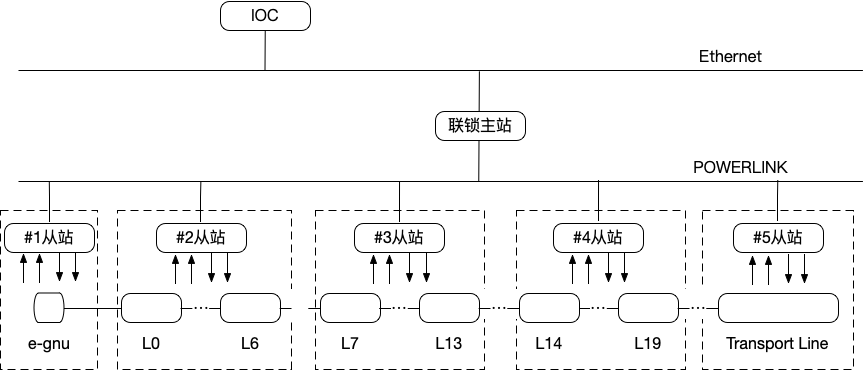
\includegraphics[width=\textwidth]{prototype-design-linac-eps.png}
	\caption{HALF直线加速器原型系统结构图}
	\label{fig:prototype-design-linac-eps}
\end{figure}

对于HALF注入器设备保护原型系统,我们可以基于第3.2节中基于POWERLINK的分布式IO测试系统的硬件设备来进行开发,设计方案如图~\ref{fig:prototype-design-linac-eps}所示。原型系统由1个联锁主站和5个联锁从站组成,主站与从站均采用基于Zynq的控制器,其中1号从站负责电子枪区域的设备安全,2号到4号从站负责监测主加速器区域内的设备安全,5号从站负责输运线区域内的设备安全。每台联锁从站有128路DI通道,负责接收相应区域内的联锁输入信号;16路DO通道负责输出相应的联锁保护信号。

主站负责处理注入器的联锁保护逻辑,主站通过千兆以太网与运行在Linux-PC上的IOC应用程序通信,主站会将来自各联锁从站的设备故障信息和联锁保护信息传输给IOC应用程序,并接收来自IOC应用程序的控制命令。

\subsection{软件开发}

原型系统的软件开发包括了联锁从站程序的开发、联锁主站程序的开发、EPICS设备驱动程序的开发和OPI的开发,下面将分别介绍程序的设计和开发。

\subsubsection{联锁从站程序的开发}

联锁从站的程序结构如图~\ref{fig:prototype-zynq-software}所示,POWERLINK协议的数据链路层和物理层基于FPGA实现,运行在ARM上的POWERLINK应用层负责处理来自“I/O module”的输入信号和来自主站的保护命令,预处理模块“Preprocess”首先对输入信号进行处理,具体包括对联锁输入信号进行旁路、锁存和复位的预处理,预处理流程如图~\ref{fig:prototype-zynq-software}所示,其中旁路和手动复位的设置是操作人员通过OPI来进行操作。预处理之后的信号会经过本地联锁算法模块“Interlock Algorithm”的处理,最后通过“Send”模块输出相应的本地保护动作,同时将与此输入信号相关的数据全部传输给主站,具体包括该信号的实时状态、预处理状态以及相关的保护信号状态。


\begin{figure}[!htb]
	\centering
	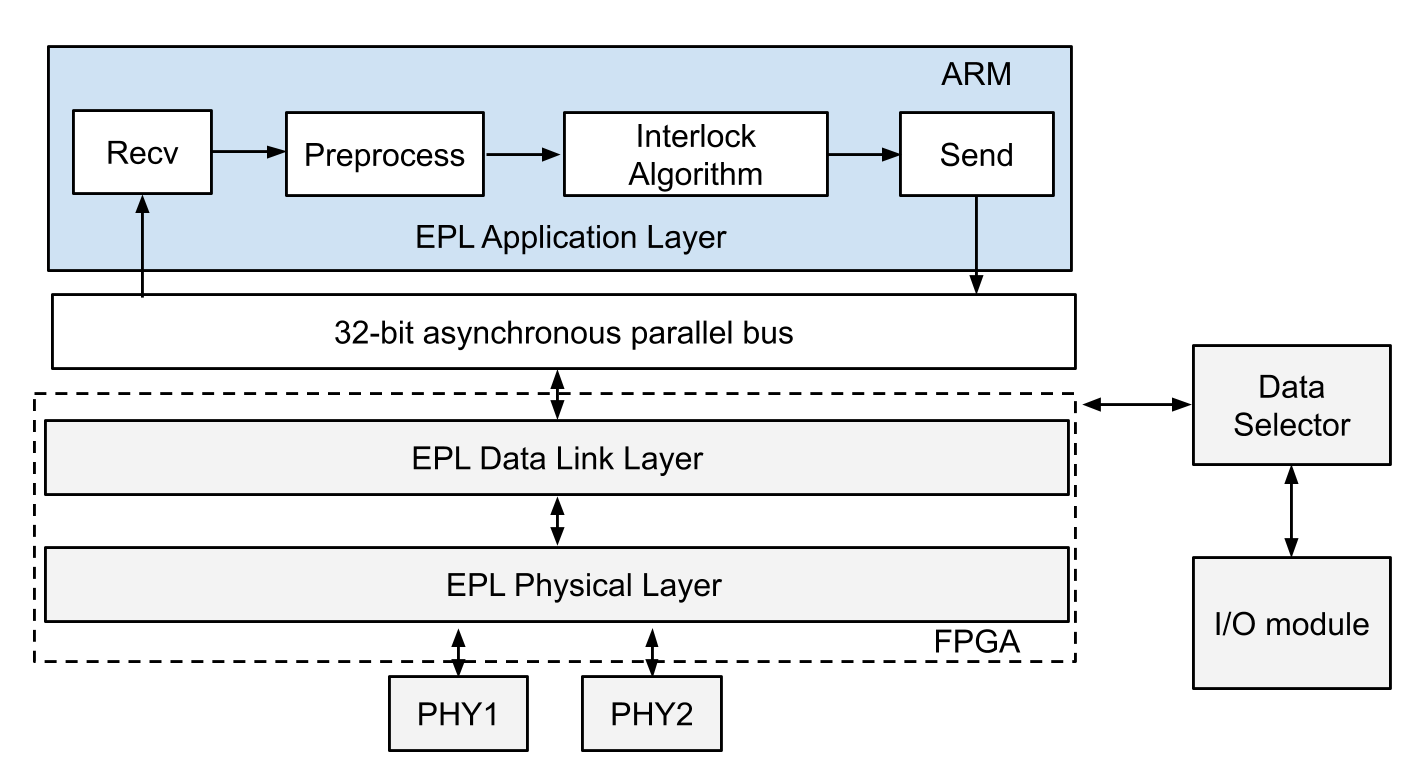
\includegraphics[width=1.1\textwidth]{prototype-zynq-software.png}
	\caption{原型系统控制器软件结构图}
	\label{fig:prototype-zynq-software}
\end{figure}


\subsubsection{联锁主站程序与EPICS设备驱动程序开发}

联锁主站的软件架构如图~\ref{fig:prototype-mn-software}所示的“MN”部分,其中POWERLINK协议的数据链路层和物理层基于FPGA实现,POWERLINK协议的应用层程序负责处理整个直线加速器各从站间的联锁逻辑。它收集来自各联锁从站的联锁输入数据,这些数据被存入“Input Data”的应用层缓存区,存储在“Input Data”中的数据将被传输到IOC应用程序,同时会“Input Data”中的数据经过“Interllock Algorithm”联锁算法功能模块之后,存入“Output Data”缓存区,被发送到相应的联锁从站输出保护。来自IOC应用程序的控制参数也存入“Output Data”缓存区,被发送到相应的联锁从站进行联锁信号的处理。 

\begin{figure}[!htb]
	\centering
	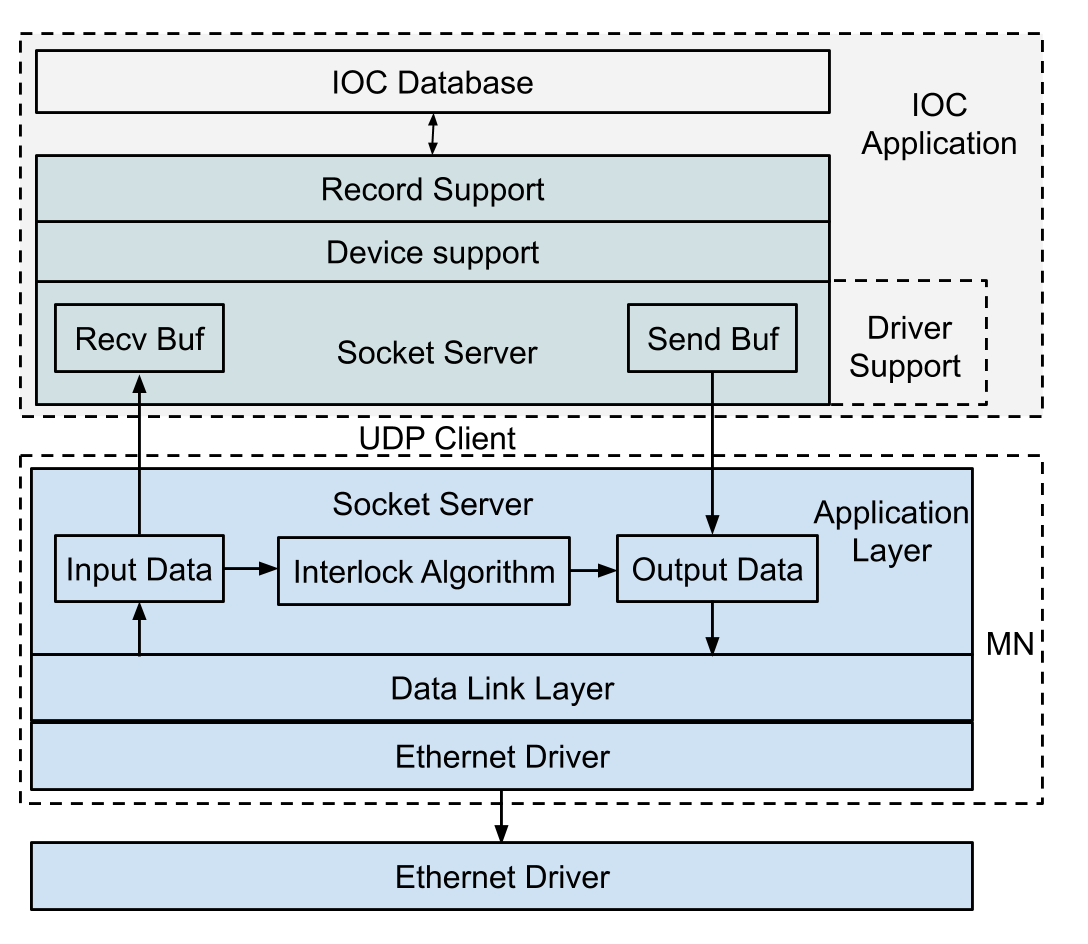
\includegraphics[width=0.8\textwidth]{prototype-mn-software.png}
	\caption{主站与IOC的软件架构}
	\label{fig:prototype-mn-software}
\end{figure}

EPICS设备驱动程序的架构如图~\ref{fig:prototype-mn-software}所示,IOC应用程序和主站之间的通信采用UDP Socket的方式,信号类型主要为数字输入和数字输出,所以可以直接采用用标准的EPICS DI和DO记录来监控设备状态信号。

\subsubsection{原型系统OPI的开发}

Phoebus/Display Builder是EPICS社区最新发布的OPI图形界面开发软件,Phoebus是用于对大规模控制系统进行监控和操作的一个软件框架和工具集,它是Control System Studio(CS-Studio)工具集的最新升级版本,不需要再依赖于Eclipse的RCP和SWT开发工具,也不再使用Workspace,提高了软件使用的方便性。我们采用Phoebus/Display Builder作为注入器设备保护原型系统的控制界面开发工具。

原型系统的OPI和IOC运行在同一台PC上,图~\ref{fig:main-panel}所示的为注入器设备保护原型系统的主界面,图中采用颜色来表示信号的状态,其中绿色表示数字信号“0”,红色表示数字信号“1”。当系统中联锁输入信号出现故障时(数字信号“1”)时,该系统图标颜色会变成深灰色,图标下的箭头会变成红色。五个保护动作图标上方的箭头颜色为红色(数字信号“1”)时,表示输出相应的保护动作,绿色(数字信号“0”)表示未实施保护。图~\ref{fig:main-panel}中所示的情况是某真空联锁信号处于故障状态,输出的保护动作包括关闭电子枪驱动光闸、禁止电子枪触发、关闭真空阀门、禁止调制器和固态放大器的触发。

\begin{figure}[!htb]
	\centering
	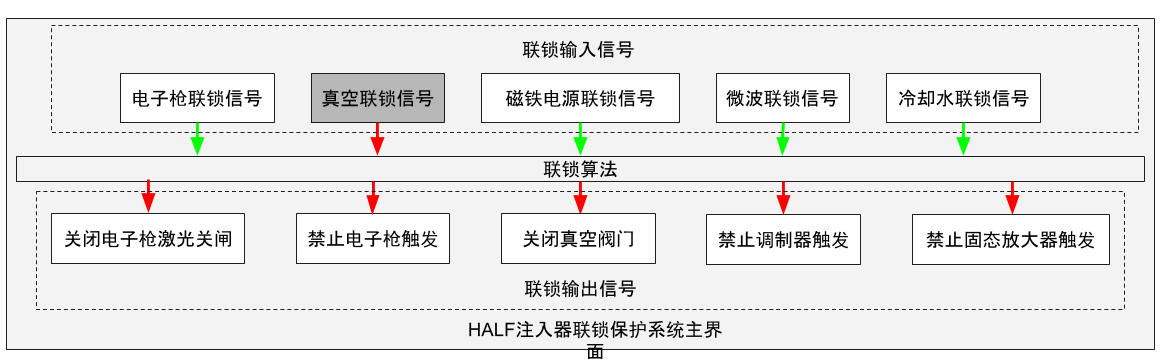
\includegraphics[width=1.1\textwidth]{main-panel.png}
	\caption{注入器设备保护系统主界面}
	\label{fig:main-panel}
\end{figure}

当点击联锁系统图标时,会弹出新界面,显示该系统中各信号的详细状态。图~\ref{fig:vacuum-panel-eps}所示的为真空联锁系统详细界面,界面分为电子枪、加速段、波导、速调管、输运线5个部分,分别详细展示了注入器各设备的真空联锁信号状态。真空联锁信号包括预警信号和报警信号,信号状态由不同的颜色来表示,红色、绿色和黑色分别表示了信号处于故障、正常或失联状态。操作人员可以直接在面板上点击旁路或复位的图标对信号进行相应的处理,图标颜色为绿色时,表示处理已开启,灰色图标表示处理已关闭。图~\ref{fig:vacuum-panel-eps}中所示的情况为,第20台速调管的真空信号(Kl-VS20)处于真空预警状态。
\\
\\
\\
\\
\\
\\
\\

\begin{figure}[!htb]
	\centering
	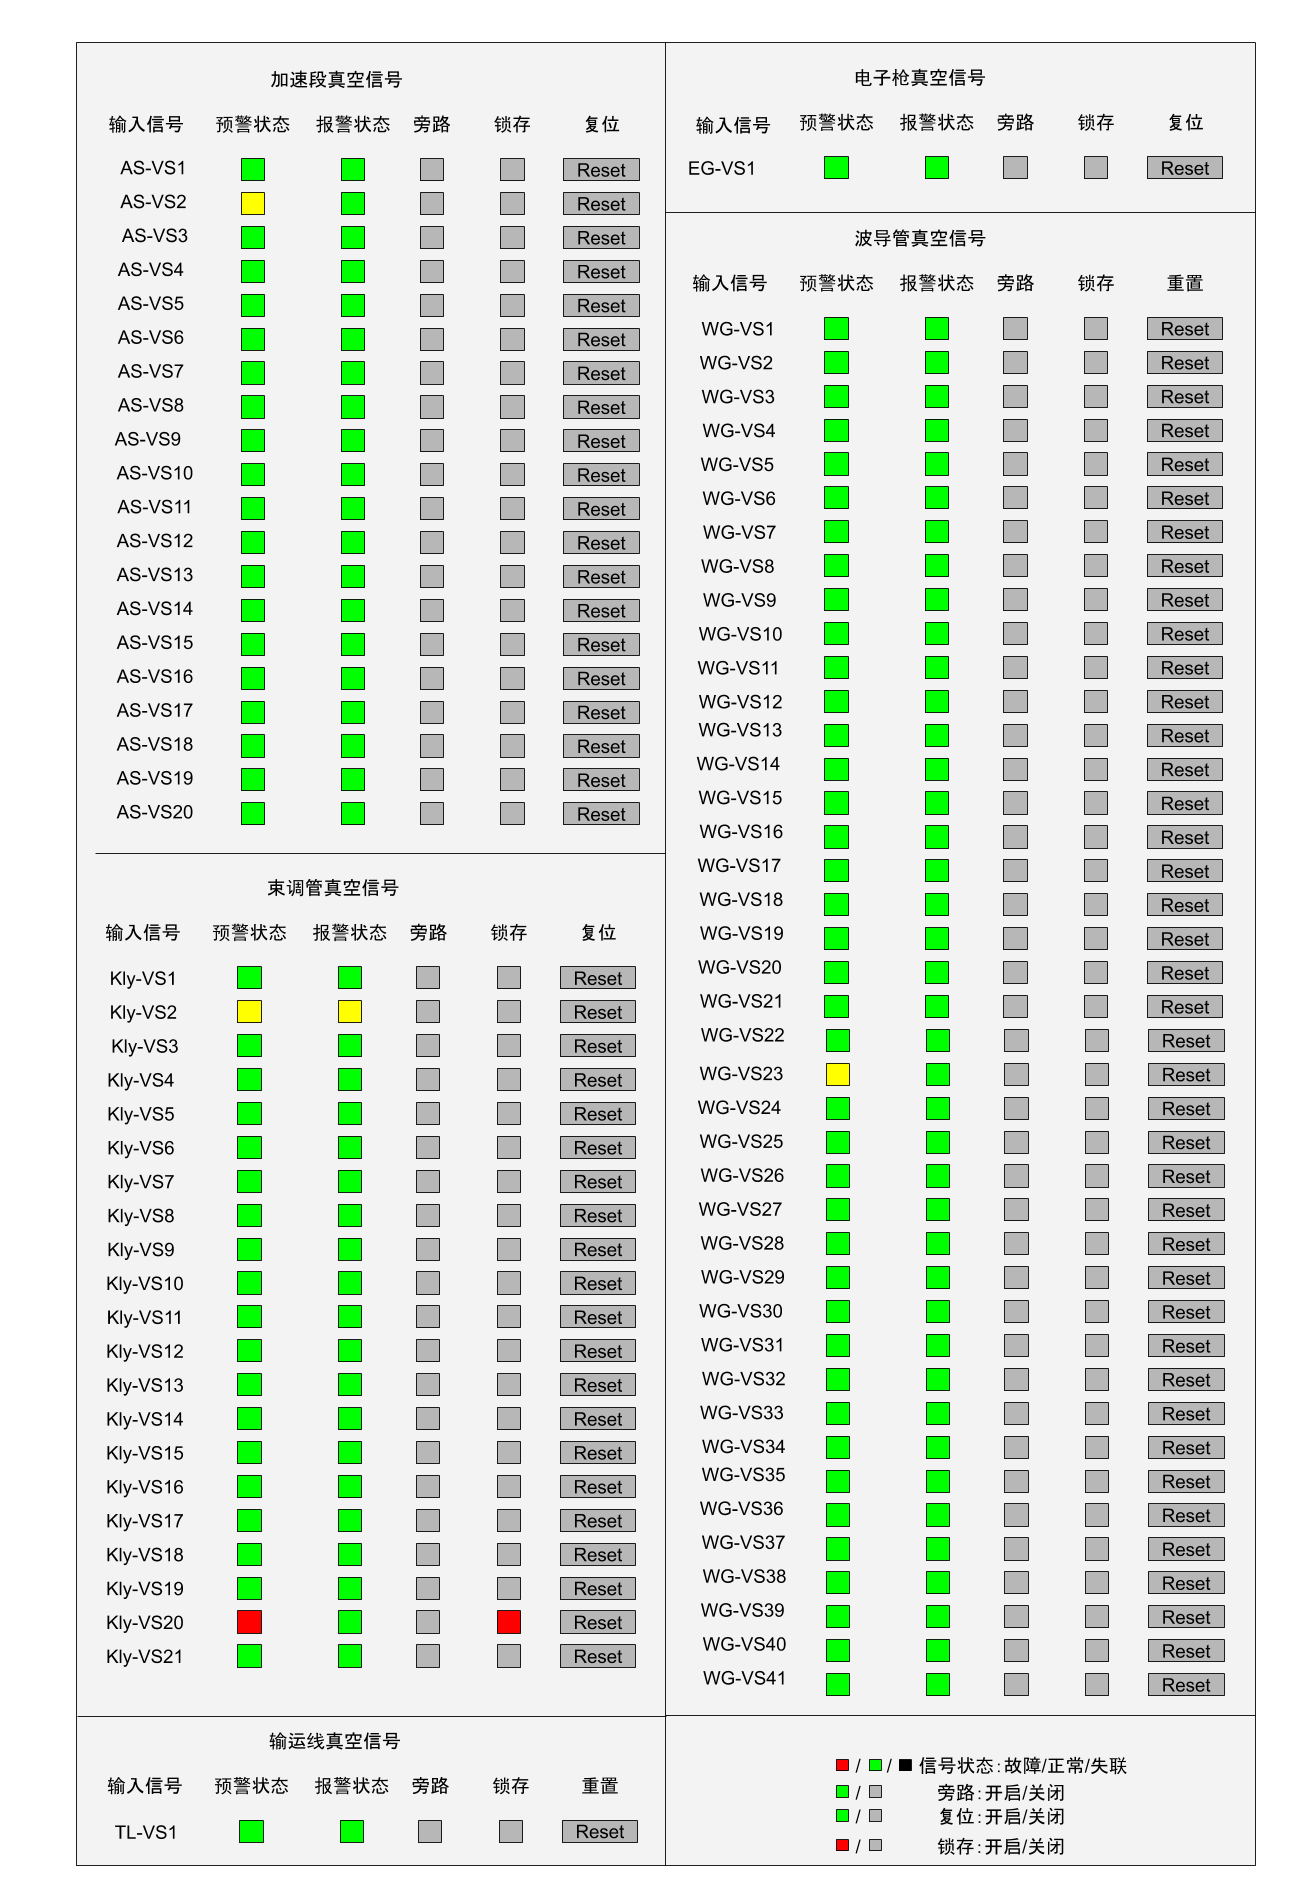
\includegraphics[width=\textwidth]{vacuum-panel-eps.png}
	\caption{真空联锁系统界面}
	\label{fig:vacuum-panel-eps}
\end{figure}

\subsection{性能测试}

原型系统的POWERLINK通信周期被配置为50$\mu$s,我们对图~\ref{fig:vacuum-panel-eps}和图~\ref{fig:main-panel}中的联锁保护场合进行了响应时间的测试,即速调管真空信号(Kl-VS20)处于真空预警状态时,此信号由4号联锁从站负责,4号从站会实施禁止相应调制器和固态放大器触发的本地联锁保护动作。同时通过主站联锁逻辑处理后,1号从站实施禁止电子枪触发信号和切断光闸的联锁保护动作。

我们将4号从站控制器的输入和输出信号连接到示波器上,以输入和输出信号的上升沿时间差来表示本地保护响应时间。测试结果如图~\ref{fig:vacuum-off}所示,Ch2(青色线)代表速调管的真空信号,Ch3(红色线)代表本地保护动作,响应时间约为5$\mu$s。

\begin{figure}[!htb]
	\centering
	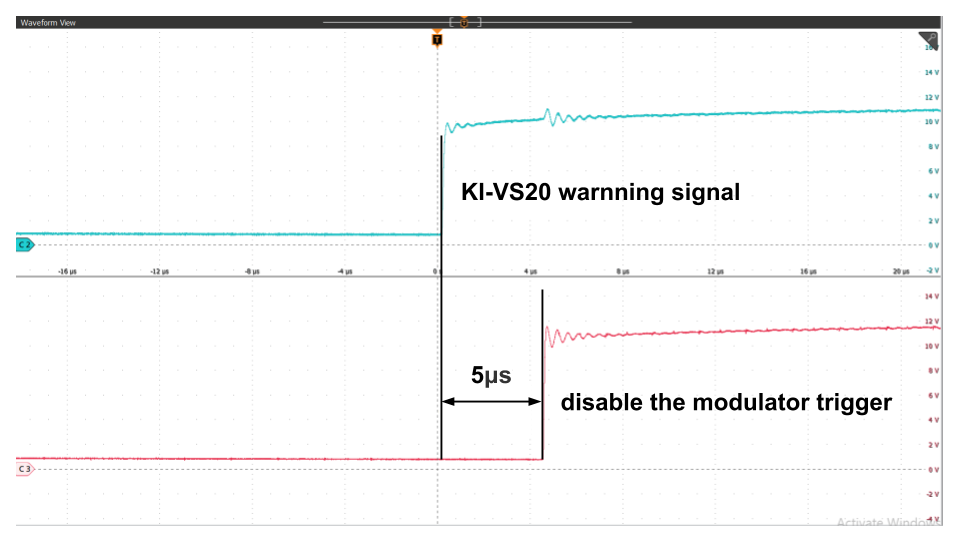
\includegraphics[width=0.8\textwidth]{vacuum-off.png}
	\caption{本地保护响应时间测试结果}
	\label{fig:vacuum-off}
\end{figure}

电子枪系统由1号联锁从站负责,我们将1号从站的输出信号和4号从站的输入信号连接到示波器上,以输入和输出信号的上升沿时间差来表示1号从站输出保护动作的响应时间。测试结果如图~\ref{fig:e-gun-trigger}所示, Ch2(青色线)代表速调管的真空信号; Ch1(黑线)代表禁止电子枪触发信号,响应时间约为160$\mu$s。

\begin{figure}[!htb]
	\centering
	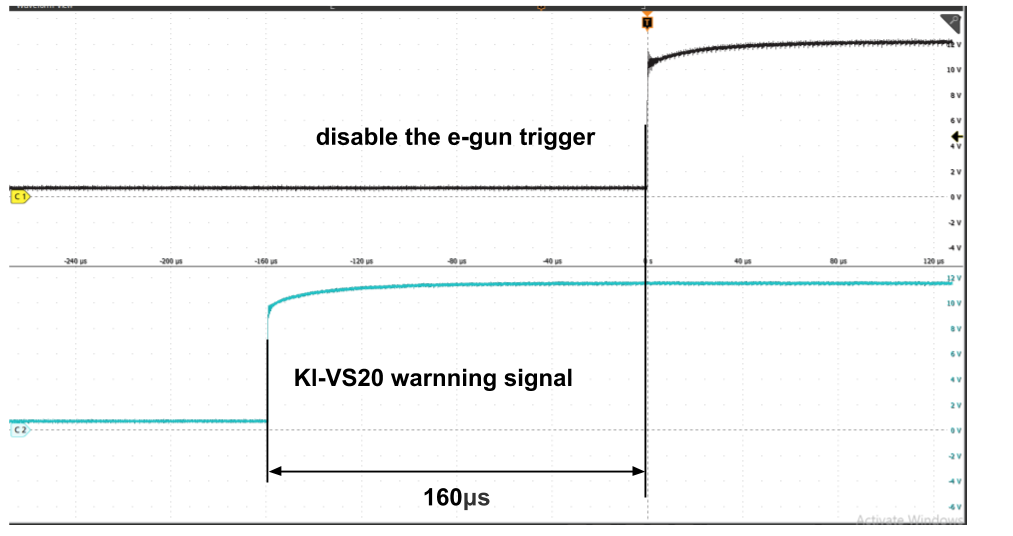
\includegraphics[width=0.8\textwidth]{e-gun-trigger.png}
	\caption{1号从站输出保护的响应时间测试结果}
	\label{fig:e-gun-trigger}
\end{figure}

\section{理论计算POWERLINK通信周期}

\label{section:理论计算POWERLINK通信周期}
通信周期直接反应系统的实时性,决定了系统的响应时间,采用理论计算和仿真建模分析两种方法来对通信周期进行对比研究,可以为不同应用场合的技术方案设计提供依据。本节首先详细分析POWERLINK通信周期的时间组成,然后结合方案2原型系统的实测数据来计算从站响应时间、HUB延时等通信参数,从而进一步完善理论计算方法,最后推导出通信周期的计算公式。

\subsection{等时同步阶段时间的理论计算}

\label{subsection:等时同步阶段时间的理论计算}

\begin{figure}[!htb]
  \centering
  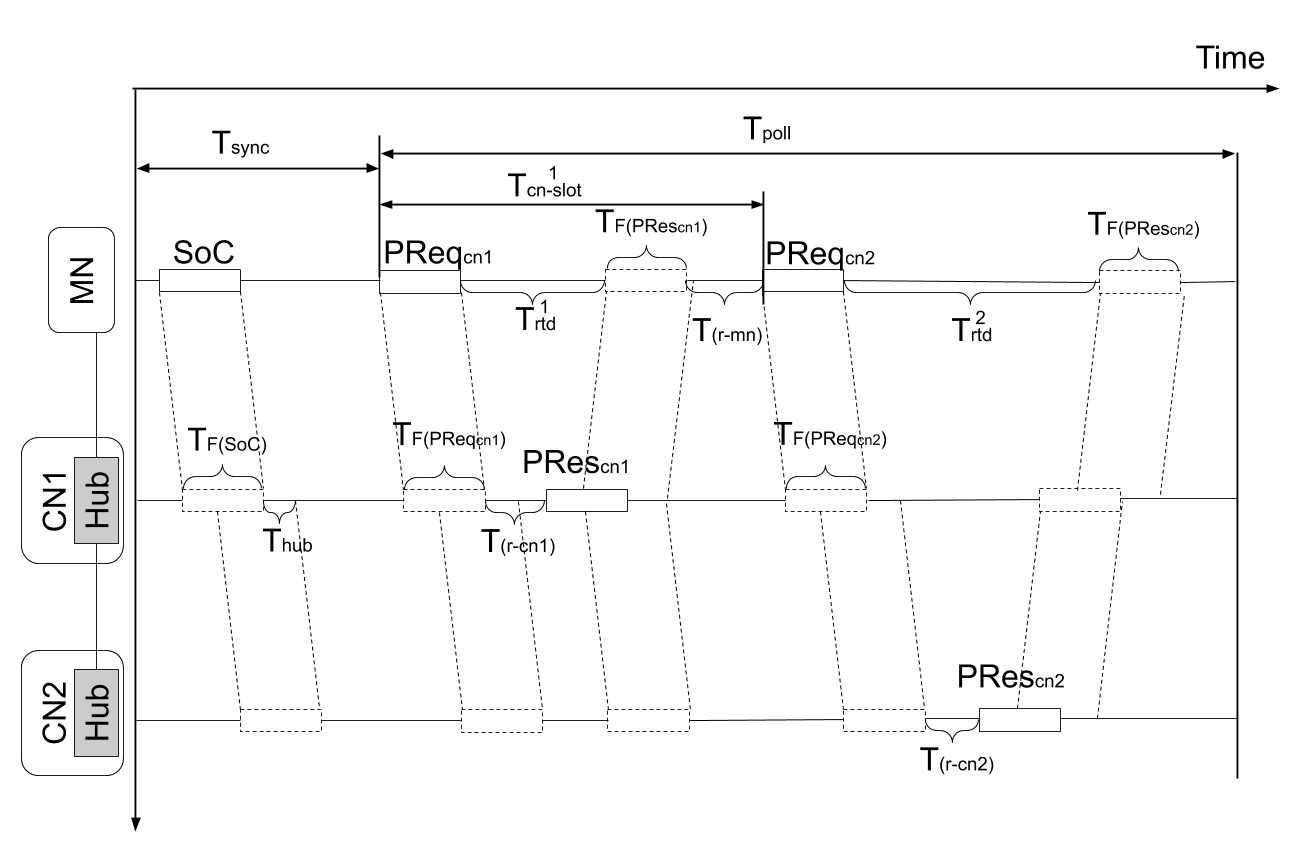
\includegraphics[width=\textwidth]{powerlink-communication-process.png}
  \caption{powerlink等时同步阶段通信过程}
  \label{fig:powerlink-communication-process}
\end{figure}

在POWERLINK通信周期中,等时同步阶段用来传输周期性的实时数据,占据了75\%以上的通信周期。图~\ref{fig:powerlink-communication-process}表示了一个基本POWERLINK网络的等时同步通信过程,该POWERLINK网络由一个主站和两个从站组成,各站点按照线型拓扑连接。等时同步阶段由同步阶段和轮询阶段组成,如公式~\ref{equation3}所示,其中$T_{ip}$代表等时同步阶段时间,$T_{sync}$和$T_{poll}$分别代表同步阶段和轮询阶段的时间。$T_{sync}$由公式~\ref{equation4}表示,$T_{F(SoC)}$为同步数据帧传输的时间。对于方案2的原型系统,SoC帧的大小为64Byte,采用千兆以太网传输,$T_{F(SoC)}$仅为0.512$\mu$s,$T_{W}$为等待从站接收并处理SoC帧的时间,从站是基于Zynq的控制器,处理速度极快。由图~\ref{fig:design2-cycle-time-test}所示,同步过程($T_{sync}$)在1$\mu$s以内可以完成,所以轮询阶段是是通信周期中耗时最长的阶段。

\begin{equation}
\label{equation3}
T_{ip}=T_{sync}+T_{poll}
\end{equation}

\begin{equation}
\label{equation4}
T_{sync}=T_{F(SoC)}+T_{W}
\end{equation}

轮询阶段时长($T_{poll}$)可由公式~\ref{equation5}表示,$T_{frames}$为轮询阶段中所有数据帧的传输时间,$T_{net}$为由所有网络组件造成的延时,网络组件包括主站、从站、HUB和网线。如图~\ref{fig:powerlink-communication-process}所示,PReq和PRes数据帧在每个从站时隙都会被发送,当主站和各从站的用户数据大小相等时,则PReq和PRes数据帧的传输时间相同均为$T_{F}$,$T_{frames}$可以用公式~\ref{equation6}表示。

\begin{equation}
\label{equation5}
T_{poll}=T_{frames}+T_{net}
\end{equation}

\begin{equation}
\label{equation6}
T_{frames}=\sum_{i=1}^n(T_{F(PReq)}^{i}+T_{F(PRes)}^{i})=2nT_{F}
\end{equation}
\begin{equation}
\label{equation7}
T_{net}=\sum_{i=1}^nT_{rtd}^{i}+nT_{r-mn}
\end{equation}

$T_{net}$由公式~\ref{equation7}表示,如图~\ref{fig:powerlink-communication-process}所示,$T_{rtd}^{i}$为主站在第i个从站时间间隙内的往返延时,$T_{r-mn}$为主站的响应时间。对于图~\ref{fig:powerlink-communication-process}所示的POWERLINK网络结构,$T_{rtd}^{1}$和$T_{rtd}^{2}$分别由公式~\ref{equation8}和~\ref{equation9}表示,其中$T_{c}$为网线传播延时,$T_{hub}$为从站控制器的HUB延时,$T_{r-cni}$为第i个从站的处理时间。根据公式~\ref{equation8}和~\ref{equation9},$T_{rtd}^{i}$可用公式~\ref{equation10}所示,因为从站设备类型相同,$T_{r-cni}$都等于$T_{r-cn}$。

\begin{equation}
\label{equation8}
T_{rtd}^{1}=2T_{c}+T_{hub}+T_{r-cn1}
\end{equation}

\begin{equation}
\label{equation9}
T_{rtd}^{2}=4T_{c}+3T_{hub}+T_{r-cn2}
\end{equation}

\begin{equation}
\label{equation10}
T_{rtd}^{i}=2iT_{c}+(2i-1)T_{hub}+T_{r-cn}
\end{equation}

\begin{equation}
\label{equation11}
\sum_{i=1}^ni=n(n+1)/2
\end{equation}

我们假设所有的从站设备类型相同且使用等长网线连接,即对于每个从站来说,参数$T_{c}$,$T_{hub}$和$T_{r-cn}$均相等。将公式~\ref{equation10}和公式~\ref{equation11}代入公式~\ref{equation7},可得公式~\ref{equation12},$T_{net}^{line}$为线性拓扑结构下所有网络组件造成的延时。

\begin{equation}
\begin{split}
\label{equation12}
T_{net}^{line}&=\sum_{i=1}^n[2iT_{c}+(2i-1)T_{hub}+T_{r-cn}]+nT_{r-mn}\\
&=n(n+1)T_{c}+n^2T_{hub}+n(T_{r-cn}+T_{r-mn})
\end{split}
\end{equation}

如图~\ref{fig:powerlink-communication-process}所示,$T_{poll}$为各从站的通信时隙$T_{cn-slot}^{i}$之和,$T_{poll}$也可以用公式~\ref{equation13}表示。根据图~\ref{fig:powerlink-communication-process}所示,$T_{cn-slot}^{i}$可用公式~\ref{equation14}表示。

\begin{equation}
\label{equation13}
T_{poll}^{i}=\sum_{i=1}^nT_{cn-slot}^{i}
\end{equation}

\begin{equation}
\label{equation14}
T_{cn-slot}^{i}=T_{F(PReq)}^{i}+T_{F(PRes)}^{i}+T_{rtd}^{i}+T_{r-mn}
\end{equation}

\section{网络模拟}
通过理论计算的分析方法,我们得到了Zynq控制器的响应时间、HUB延时等通信参数,并初步推导出了等时同步阶段时长的计算公式。为了对更大规模的POWERLINK方案进行准确可靠的评估,我们还发展了仿真建模的分析方法。POWERLINK网络仿真基于OMNet++网络模拟器展开,我们首先建立了支持千兆POWERLINK通信的节点模型,然后通过对原型系统进行仿真来验证仿真建模分析方法的可行性,最后通过仿真建模的分析方法对大规模的POWERLINK方案进行性能评估。

OMNeT++(Objective Modular Network Testbed in C++)是一个开源可扩展的、模块化、基于组件的C++仿真库和框架,主要用于构建网络仿真器。作为面向对象的离散事件仿真器,OMNeT++主要用于通信网络和分布式系统的仿真。OMNeT++的主要组成部分如下:

\begin{enumerate}
  \item 仿真内核库:OMNeT++提供的仿真类库代码;
  \item 网络拓扑描述文件:由NED语言编写的文件,既可以用来描述网络拓扑结构,又可以通过参数、门、信道连接、简单模块等来定义复杂模块;
  \item 消息定义文件:用于定义数据报文格式;
  \item 简单模块定义文件:简单模块的行为定义文件,包括C++编写的*.cc文件和*.h
  \item 用户接口:该接口用于仿真运行时的测试,演示等工作。
\end{enumerate}

在使用OMNeT++建模中,最常使用的就是INET框架。INET框架是开源的OMNeT++的标准协议模型库,对应OMNeT的各种新版本INET框架还在不断更新中,INET框架包含了常用的多种有线和无线协议的模型,具体到各种物理层模型、应用层模型等。在POWERLINK仿真建模中,我们使用的是OMNeT++4.6版本搭配inet-2.6-b673687版本。

\subsection{POWERLINK通信节点建模}

\begin{figure}[!htb]
  \centering
  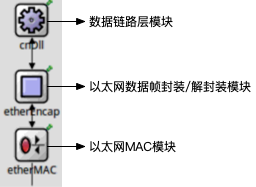
\includegraphics[width=0.6\textwidth]{powerlink-model.png}
  \caption{POWERLINK通信节点模型}
  \label{fig:powerlink-model}
\end{figure}
基于OMNeT++仿真平台,我们对POWERLINK主站和从站进行了建模。节点模型如图~\ref{fig:powerlink-model}所示,由以下三个模块组成:

\begin{enumerate}
  \item 以太网MAC模块:采用INET框架下的标准以太网MAC模块,支持千兆以太网通信;
  \item 以太网数据帧封装/解封装模块:采用INET框架下的EtherEncap模块,用于EthernetII数据帧的封装和解封装;
  \item 数据链路层模块:按照POWERLINK的SCNM机制定义了模块行为。
\end{enumerate}

除了对通信节点建模之外,还定义了FPGAHUB模块用于数据帧的转发,采用INET框架下的Eth1G千兆以太网模块用于连接各节点,在.msg文件中定义四种POWERLINK数据帧结构。

\section{理论计算POWERLINK通信周期}

\label{section:理论计算POWERLINK通信周期}
通信周期直接反应系统的实时性,决定了系统的响应时间,采用理论计算和仿真建模分析两种方法来对通信周期进行对比研究,可以为不同应用场合的技术方案设计提供依据。本节首先详细分析POWERLINK通信周期的时间组成,然后结合方案2原型系统的实测数据来计算从站响应时间、HUB延时等通信参数,从而进一步完善理论计算方法,最后推导出通信周期的计算公式。

\subsection{等时同步阶段时间的理论计算}

\label{subsection:等时同步阶段时间的理论计算}

\begin{figure}[!htb]
  \centering
  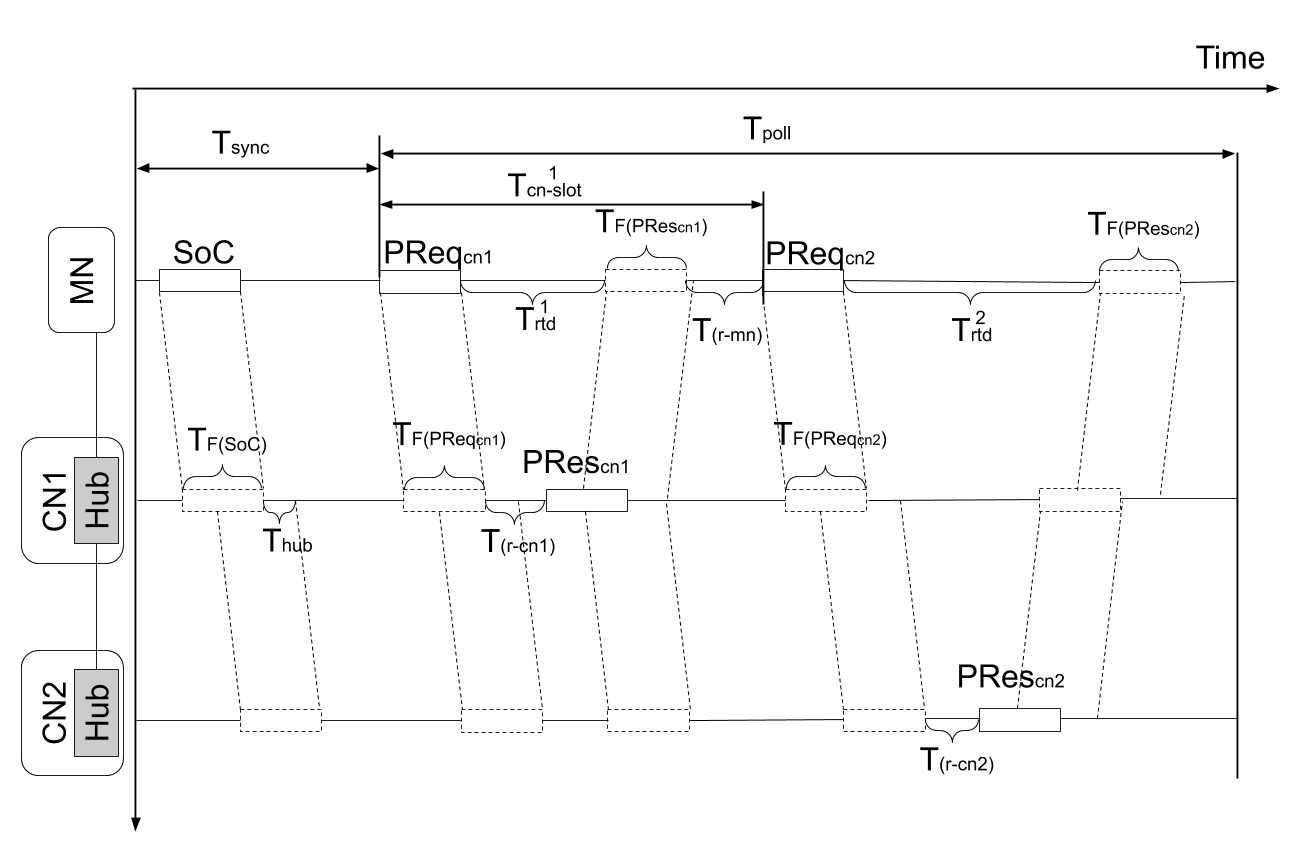
\includegraphics[width=\textwidth]{powerlink-communication-process.png}
  \caption{powerlink等时同步阶段通信过程}
  \label{fig:powerlink-communication-process}
\end{figure}

在POWERLINK通信周期中,等时同步阶段用来传输周期性的实时数据,占据了75\%以上的通信周期。图~\ref{fig:powerlink-communication-process}表示了一个基本POWERLINK网络的等时同步通信过程,该POWERLINK网络由一个主站和两个从站组成,各站点按照线型拓扑连接。等时同步阶段由同步阶段和轮询阶段组成,如公式~\ref{equation3}所示,其中$T_{ip}$代表等时同步阶段时间,$T_{sync}$和$T_{poll}$分别代表同步阶段和轮询阶段的时间。$T_{sync}$由公式~\ref{equation4}表示,$T_{F(SoC)}$为同步数据帧传输的时间。对于方案2的原型系统,SoC帧的大小为64Byte,采用千兆以太网传输,$T_{F(SoC)}$仅为0.512$\mu$s,$T_{W}$为等待从站接收并处理SoC帧的时间,从站是基于Zynq的控制器,处理速度极快。由图~\ref{fig:design2-cycle-time-test}所示,同步过程($T_{sync}$)在1$\mu$s以内可以完成,所以轮询阶段是是通信周期中耗时最长的阶段。

\begin{equation}
\label{equation3}
T_{ip}=T_{sync}+T_{poll}
\end{equation}

\begin{equation}
\label{equation4}
T_{sync}=T_{F(SoC)}+T_{W}
\end{equation}

轮询阶段时长($T_{poll}$)可由公式~\ref{equation5}表示,$T_{frames}$为轮询阶段中所有数据帧的传输时间,$T_{net}$为由所有网络组件造成的延时,网络组件包括主站、从站、HUB和网线。如图~\ref{fig:powerlink-communication-process}所示,PReq和PRes数据帧在每个从站时隙都会被发送,当主站和各从站的用户数据大小相等时,则PReq和PRes数据帧的传输时间相同均为$T_{F}$,$T_{frames}$可以用公式~\ref{equation6}表示。

\begin{equation}
\label{equation5}
T_{poll}=T_{frames}+T_{net}
\end{equation}

\begin{equation}
\label{equation6}
T_{frames}=\sum_{i=1}^n(T_{F(PReq)}^{i}+T_{F(PRes)}^{i})=2nT_{F}
\end{equation}
\begin{equation}
\label{equation7}
T_{net}=\sum_{i=1}^nT_{rtd}^{i}+nT_{r-mn}
\end{equation}

$T_{net}$由公式~\ref{equation7}表示,如图~\ref{fig:powerlink-communication-process}所示,$T_{rtd}^{i}$为主站在第i个从站时间间隙内的往返延时,$T_{r-mn}$为主站的响应时间。对于图~\ref{fig:powerlink-communication-process}所示的POWERLINK网络结构,$T_{rtd}^{1}$和$T_{rtd}^{2}$分别由公式~\ref{equation8}和~\ref{equation9}表示,其中$T_{c}$为网线传播延时,$T_{hub}$为从站控制器的HUB延时,$T_{r-cni}$为第i个从站的处理时间。根据公式~\ref{equation8}和~\ref{equation9},$T_{rtd}^{i}$可用公式~\ref{equation10}所示,因为从站设备类型相同,$T_{r-cni}$都等于$T_{r-cn}$。

\begin{equation}
\label{equation8}
T_{rtd}^{1}=2T_{c}+T_{hub}+T_{r-cn1}
\end{equation}

\begin{equation}
\label{equation9}
T_{rtd}^{2}=4T_{c}+3T_{hub}+T_{r-cn2}
\end{equation}

\begin{equation}
\label{equation10}
T_{rtd}^{i}=2iT_{c}+(2i-1)T_{hub}+T_{r-cn}
\end{equation}

\begin{equation}
\label{equation11}
\sum_{i=1}^ni=n(n+1)/2
\end{equation}

我们假设所有的从站设备类型相同且使用等长网线连接,即对于每个从站来说,参数$T_{c}$,$T_{hub}$和$T_{r-cn}$均相等。将公式~\ref{equation10}和公式~\ref{equation11}代入公式~\ref{equation7},可得公式~\ref{equation12},$T_{net}^{line}$为线性拓扑结构下所有网络组件造成的延时。

\begin{equation}
\begin{split}
\label{equation12}
T_{net}^{line}&=\sum_{i=1}^n[2iT_{c}+(2i-1)T_{hub}+T_{r-cn}]+nT_{r-mn}\\
&=n(n+1)T_{c}+n^2T_{hub}+n(T_{r-cn}+T_{r-mn})
\end{split}
\end{equation}

如图~\ref{fig:powerlink-communication-process}所示,$T_{poll}$为各从站的通信时隙$T_{cn-slot}^{i}$之和,$T_{poll}$也可以用公式~\ref{equation13}表示。根据图~\ref{fig:powerlink-communication-process}所示,$T_{cn-slot}^{i}$可用公式~\ref{equation14}表示。

\begin{equation}
\label{equation13}
T_{poll}^{i}=\sum_{i=1}^nT_{cn-slot}^{i}
\end{equation}

\begin{equation}
\label{equation14}
T_{cn-slot}^{i}=T_{F(PReq)}^{i}+T_{F(PRes)}^{i}+T_{rtd}^{i}+T_{r-mn}
\end{equation}


